\chapter{EcoBuilder}
\label{chap:joy}

\begin{figure}
    \centering
    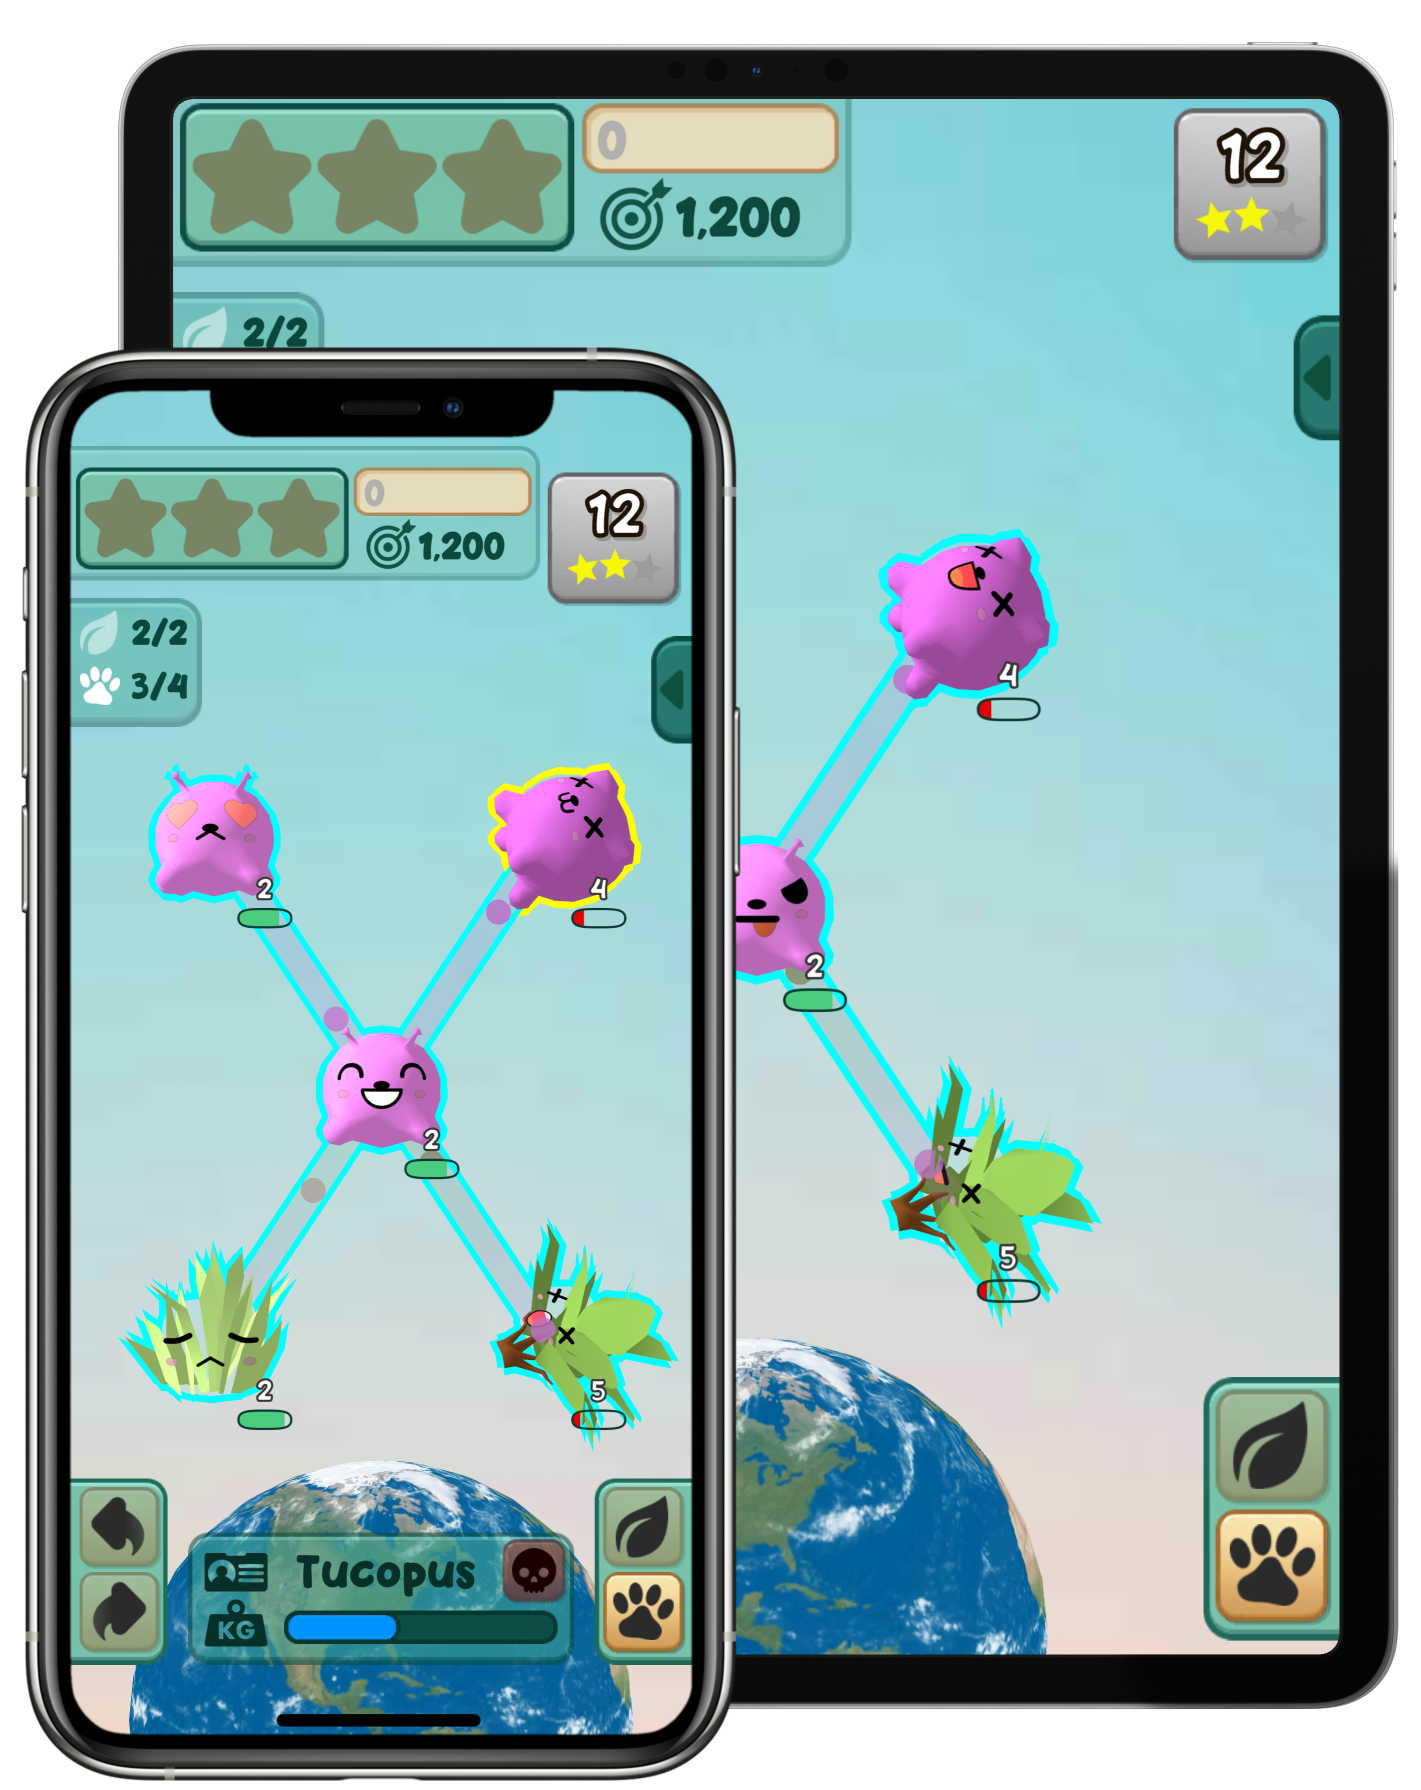
\includegraphics[width=\textwidth]{joy/device.png}
    \caption[EcoBuilder displayed on two mobile devices.]{Screenshots of EcoBuilder displayed on an iPhone and an iPad. The particular ecosystem shown depicts the bottom-right plant going extinct due to apparent competition, as well as the top-right animal going extinct due to competitive exclusion.}
    \label{fig:ecobuilder_device}
\end{figure}

The preceding chapters focused on the algorithms and methods underlying visualisation techniques, but it is important to remember that visualisation is a discipline with practical applications firmly in mind as the end goal.
The work in this chapter will explore such a goal to move towards an engineering focus, specifically the design and development of \emph{EcoBuilder}, a research-oriented video game about building ecosystems.

\section{Background}
\label{sec:joy_background}
The unique selling point of EcoBuilder is that its ecosystem simulation is based on the same mathematical models studied by theoretical ecologists. The review of background literature in this section will therefore begin by discussing the models chosen in the following Section~\ref{sec:predator_prey}. With the knowledge of \emph{how} pairs of species interact with each other, the following Section~\ref{sec:topology} will study the choice of \emph{which} species interact at all. Section~\ref{sec:citizen_science} will outline a brief history of previous attempts to crowdsource research through the citizen science approach, and give context to why EcoBuilder was created.

\subsection{Predator--prey interactions}
\label{sec:predator_prey}
Ever since Isaac Newton formulated his physical laws of motion, it has become clear that nature speaks in the language of differential equations. From simple mechanical systems such as the oscillating swing of a pendulum \cite{Fulcher1976}, to the cosmic dance of celestial bodies in space \cite{Marchal2012}, and even the electrical action potentials across every neuron in the brain that is deciding which words should go into this sentence \cite{Hodgkin1952}, calculus has time and again been an invaluable tool for describing the natural world. 

The behaviour of species ecosystems is no different, where the most widely used models are function by defining the change in abundance (measured by biomass per unit area) over time.
There are many such examples of this, ranging from the simple and linear systems to be studied here, to highly complex data-driven models such as \emph{EcoPath with EcoSim}, which has been used for decades to inform environmental policy for aquatic conservation \cite{Christensen2004}.
Other models include ones that consider the effects of temperature on metabolic rate \cite{Savage2004, Dell2014}, spatio-temporal dynamics such as turbulance in water \cite{Watteaux2015}, or evolution to produce the correct dynamics as an emergent property \cite{Laird2008}

But perhaps the oldest and most commonly studied of these models is known as the Lotka-Volterra equations, defined as
\begin{equation}
  \frac{d\mathbf{z}_i}{dt} = \mathbf{z}_i(\mathbf{r}_i + \sum_j\mathbf{A}_{ij}\mathbf{z}_j)
  \label{eq:lotka_volterra}
\end{equation}
where $\mathbf{d}_i$ is the abundance of species $i$, $\mathbf{r}_i$ is its growth rate (or death rate if it is negative), and $\mathbf{A}_{ij}$ is the strength of the interaction between two species, which is positive if $i$ eats $j$ and negative if $j$ eats $i$. 
This can be written to include all species simultaneously as
\begin{equation}
    \frac{d\mathbf{z}}{dt} = \mathbf{z}(\mathbf{r} + \mathbf{Az}).
    \label{eq:interaction_matrix}
\end{equation}
The matrix $\mathbf{A}$ is known as the \emph{interaction matrix}, and is called that because it contains all the information on how each pair of species interact with each other.
There are five classifications of interaction possible in such a model, designated by the nature of the values in the corresponding pair of values in this matrix. For example, if $\mathbf{A}_{ij}>0$ and $\mathbf{A}_{ji}<0$, then it is a standard example of species $i$ preying on species $j$, where the `sign' of the interaction is $(+,-)$. The remaining types are mutualism $(+,+)$, competition $(-,-)$, commensalism $(+,0)$, and amensalism $(-,0)$.
Different models include differing amounts of each type of interaction, and the proportion of types can strongly influence the behaviour of the system \cite{Tang2014Correlation}. However the predator--prey type is the most commonly studied and most prevalent in nature, and so will be the only one considered here.

The purpose of the above equations is to use them to find values of $\mathbf{x}$, and the standard way of doing this for differential equations is to simulate by performing numerical integration at each time step, using methods such as Runge-Kutta \cite{Press2007Runge}.\footnote{This was used in older versions of the game, but brings with it numerical problems such as stiff equations leading to instability \cite{Press2007Runge}, or having to choose a suitable integration time step. It also adds the issue of having to choose an arbitrary abundance threshold for species to go extinct.}
However the simplicity of the model chosen allows something different: it can be analytically solved for an \emph{equilibrium} point. This is the solution at which the interactions fully balance each other such that the instantaneous change in abundance is zero. Note the similarity of this method to the graph layout algorithm of Tutte shown in Section~\ref{sec:nodes_background}, Equation~\eqref{eq:tutte}.
This is done by setting the left-hand side of Equation~\eqref{eq:interaction_matrix} to zero, where it is clear that the system contains many trivial solutions with any species $x=0$, which corresponds to the natural case of an extinct species staying extinct.
Since the solution at which every species has non-zero abundance is one of interest, the $\mathbf{x}$ outside bracket is simply cancelled out to reach the solution
\begin{equation}
  \mathbf{z^*} = -\mathbf{A}^{-1}\mathbf{r}.
  \label{eq:equilibrium}
\end{equation}
where $\mathbf{z}^*$ is the strictly non-zero abundances of every species at equilibrium.
This is equivalent to a linear system of equations and so can be solved exactly by numerical methods.
If the solution $\mathbf{z^*}$ contains any negative numbers the system of equations is said to not be \emph{feasible} i.e.\ it is not possible for all species to coexist.

\subsubsection{Local asymptotic stability}
If the system is feasible, another benefit of this technique is that it allows for the derivation of the \emph{local asymptotic stability} of this fixed point, which has been widely used in the literature as a mathematically elegant and computationally tractable measure of the stability of food webs~\cite{May1973, Emmerson2004}. This definition will be henceforth referred to simply as stability. 
To find if a system is stable, the first step is to find the Jacobian matrix
\begin{equation}
  \mathbb{J} = \begin{bmatrix}
    \frac{\partial f_1}{\partial \mathbf{z}_1} & 
    \cdots &
    \frac{\partial f_1}{\partial \mathbf{z}_n} \\
    \vdots &
    \ddots &
    \vdots \\
    \frac{\partial f_n}{\partial \mathbf{z}_1} & 
    \cdots &
    \frac{\partial f_n}{\partial \mathbf{z}_n}
  \end{bmatrix}
\end{equation}
where $f_i$ is the right side of Equation~\eqref{eq:lotka_volterra} and $n=|V|$ is the total number of species (vertices) in the food web (graph).
This is the matrix of all possible partial derivatives of a system, which describes the instantaneous behaviour of the system by linearising it. This Jacobian is then evaluated at the feasible equilibrium point $\mathbf{z}^*$, resulting in what is known as a \emph{community matrix}. For the Lotka-Volterra equations studied here, this is
\begin{equation}
  \mathbb{J}|_\mathbf{z^*} = \begin{bmatrix}
    \mathbf{r}_1 + 2\mathbf{A}_{11}\mathbf{z}_1^* + \sum_{i\neq 1}^n\mathbf{A}_{1i}\mathbf{z}_i^*
    \;\cdots\;
    \mathbf{A}_{1n}\mathbf{z}_1^*\\
    \vdots 
    \qquad\qquad\quad\;\;\ddots\qquad\qquad\quad\;\;
    \vdots \\
    \mathbf{A}_{n1}\mathbf{z}_n^*
    \;\cdots\;
    \mathbf{r}_n + 2\mathbf{A}_{nn}\mathbf{z}_n^* + \sum_{i\neq n}^n\mathbf{A}_{ni}\mathbf{z}_i^* 
  \end{bmatrix}
  \label{eq:jacobian_evaluated}
\end{equation}
which also conveniently simplifies to $\mathbb{J}|_\mathbf{z^*} = \mathrm{diag}(\mathbf{z^*})\mathbf{A}$, after substituting $\mathbf{z^*}$ back in using Cramer's rule \cite{May1973}.
The system can then be declared locally stable if the largest real part of any eigenvalue of the community matrix is non-negative
\begin{equation}
    \Lambda \leq 0.
    \label{eq:lambda_stability}
\end{equation}
% In fact the further away from zero $\Lambda$ is, the quicker the system returns to the equilibrium point $\mathbf{x}^*$ after a perturbation, and therefore the more resilient the ecosystem is.
An intuitive physical interpretation of this type of stability can be seen by imagining the two ways of holding a chopstick vertically when gripping only a single end. If the chopstick is pointing upwards, even the slightest nudge will make it fall over due to gravity. If it is dangling downwards, gravity will reset its position after a nudge, and it can be called stable.
In the context of ecosystems, the chopstick is a species, and the nudge is an environmental perturbation such as a natural disaster or invading species.

The behaviour of the community matrix $\mathbb{J}|_\mathbf{z^*}$ is what is usually studied in mathematical ecology, due to the fact that it can be reverse-engineered to apply to almost any system of differential equations. It therefore sidesteps the problem of choosing which model to use, by jumping straight to this matrix.
It is also the source of the long standing `complexity vs.\ stability' debate in the world of ecology, because it can be shown that as the number of species, i.e.\ size of $\mathbf{A}$, grows, the chance of Equation~\eqref{eq:lambda_stability} being satisfied tends to zero, even for small ecosystems of only a few dozen species \cite{May1973}.
The reason for the debate is that systems exist in the real world with many more species than the math suggests is possible, and many subsequent works have studied what features of ecosystems allow such a contradiction to occur.
For example, Tang et al.\ \cite{Tang2014Correlation} show that the correlation between pairs of elements in $\mathbf{A}$ can improve stability, Brose et al.\ \cite{Brose2006} study the consequences of body mass, and Johnson et al.\ \cite{Johnson2014} study the layered nature of groups of species.

However a common criticism is that this method assumes the existence of a feasible equilibrium in the first place, and this is far from guaranteed. It has also been showed that in simple systems like the Lotka-Volterra equations studied here, that feasibility almost always leads to stability anyway \cite{Dougoud2018}. For this reason, the work done here will focus solely on feasibility, where nevertheless any results found can also apply to stability.

% We plan on using \eqref{eq:lambda_stability} directly within the game as one of the possible metrics for a high-score.
% Other possible metrics include the total energy flow (flux) of the system, the trophic height (largest trophic level), or the reactivity of the fixed point~\cite{Tang2014Reactivity}.
% All of the three solutions just described have been implemented into the game and an early screenshot can be seen in Figure~\ref{screenshot}.

% As we shall see, this also solves our issue of having to choose a suitable extinction threshold, as well as having to integrate differential equations for a long time after the game ends to make sure that species slowly on their way to extinction do not count towards the player score.


\subsubsection{Metabolic scaling}
The steps so far have discussed how to find abundances given the interaction matrix $\mathbf{A}$, but it has not yet been discussed how to find the numerical values to go into the matrix in the first place, i.e.\ its parameterisation.
To fill this gap, a methodology known as \emph{metabolic scaling} will be used. It leverages the idea that each species has a metabolism rate that can be measured, i.e.\ the speed at which an organism converts a food source into either energy for movement or materials for growth. For plants this involves mainly converting nutrients and sunlight into biomass, and for animals this involves mainly converting biomass into movement to hunt prey.

\begin{figure}
    \centering
    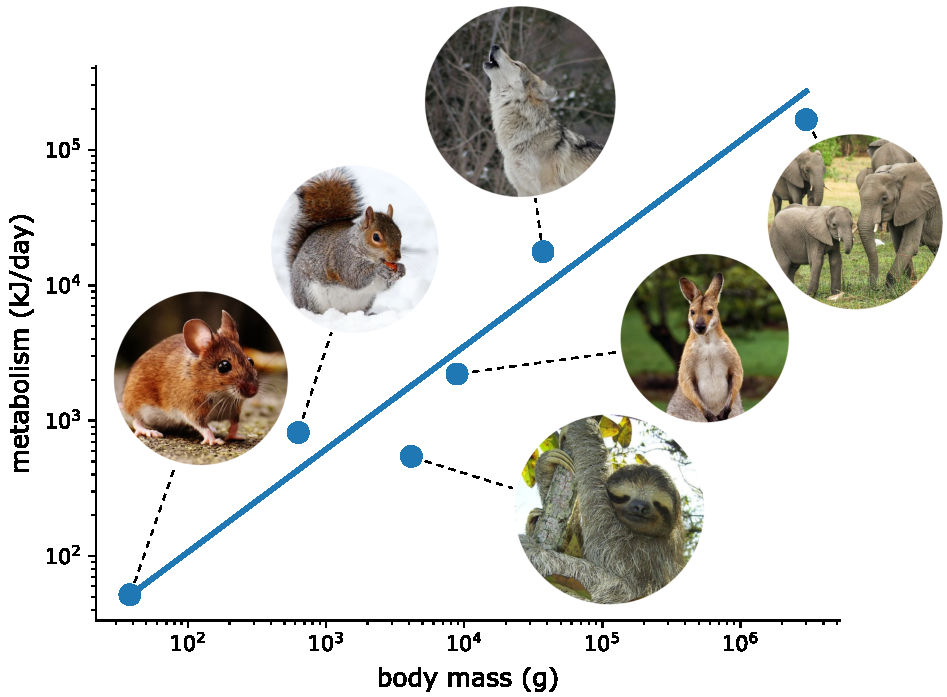
\includegraphics[width=.8\textwidth]{joy/metabolism.pdf}
    \caption[A plot of metabolism against individual body mass]{A plot of metabolism against individual body mass for a selection of animals. Note the outlier position of the sloth, showing that the model is imperfect, but still a very good estimate when considering the complexity of life. Data taken from \cite{Nagy1999}, power law slope and intercept from \cite[Fig.~2]{Brown2004}.}
    \label{fig:metabolism}
\end{figure}

Metabolism is useful for two main reasons. The first is that, as it essentially measures the energy output of a species, it is strongly correlated with other traits such as movement speed \cite{Hirt2017} and therefore has been successfully used for parameterisation of $\mathbf{A}$ \cite{Savage2004, Vucic-Pestic2010, Pawar2015}. The second is that metabolism can be closely estimated through an inverse relationship to individual body mass, a connection that has been empirically measured and verified \cite{Brown2004}. The study of the relationships between mass and other biological traits is known as \emph{allometry}. Some examples of species and their metabolisms can be seen in Figure~\ref{fig:metabolism}.

Specifically, the allometric functions used for the reproduction rates $\mathbf{r}$ in Equation~\eqref{eq:lotka_volterra} are
\begin{equation}
  \mathbf{r}_i =
  \begin{cases}
    \;b_0\mathbf{m}_i^{\beta-1} & \text{if $i$ is producer}\\
    \;-d_0\mathbf{m}_i^{\beta-1} & \text{if $i$ is consumer}
  \end{cases}
  \label{eq:metabolism_beta}
\end{equation}
where $b_0$ and $d_0$ are constants to normalise birth and death rates, and $\mathbf{m}_i$ is the body mass of species $i$ in kilograms. The exponent $\beta$ is a empirically verified relationship between metabolism and individual body mass \cite{Brown2004}, and it is taken minus one in order to convert it into mass-specific units.
Remarkably, the same exponent of $\beta=\sfrac{3}{4}$ can be applied to species of all sizes, from the smallest bacteria to the largest blue whale \cite{Kleiber1947}. It is theorised to take a value of $\sfrac{3}{4}$ --- rather than the $\sfrac{2}{3}$ that one would expect from a spherical surface area to volume ratio --- due to the fractal spreading pattern of tubes (such as veins) \cite{West1997}, although not without controversy \cite{Agutter2004}.

The interaction strengths of predator--prey interactions are defined as
\begin{equation}
  \mathbf{A}_{ij} =
  \begin{cases}
    \;-a_0\mathcal{F}(i,j)\mathbf{m}_j^{\text{--}1} & \text{if $i$ is prey}\\
    \;e_0a_0\mathcal{F}(j,i)\mathbf{m}_i^{\text{--}1} & \text{if $i$ is predator}
  \end{cases}
  \label{eq:interaction_strength}
\end{equation}
where $a_0$ is a normalising constant, $e_0$ measures biomass conversion efficiency, and $\mathcal{F}(i,j)$ is a function describing the rate at which an individual predator comes into contact with its prey. The $\mathbf{m}^{\text{--}1}$ factor at the end is to account for individuality and convert it into mass-specific units, just as the minus one in the exponent of Equation~\eqref{eq:metabolism_beta}.
The function $\mathcal{F}(i,j)$ can be expressed in many ways, and is more difficult to measure than individual metabolism as it involves the interaction between two species. To overcome this, Pawar et al.\ \cite{Pawar2012} constructed an allometric model that simulates species as randomly moving individuals, such that they can be treated as particles colliding under a Brownian motion approximation \cite{Ocubo1980}. Traits such as movement speed and eye strength all also have allometric relationships, and so were carefully combined (and validated against empirical data) to construct a mechanistic model of species interaction.
The final resulting formulations for $\mathcal{F}(i,j)$ are
\begin{equation}
  \mathcal{F}(i,j) =
  \begin{cases}
    \;\mathbf{m}_j^{p_v+2p_d} \sqrt{1+\left(\frac{\mathbf{m}_i}{\mathbf{m_j}}\right)^{2p_v}}\left(\frac{\mathbf{m}_i}{\mathbf{m}_j}\right)^{p_d} & \text{if active capture}\\
    \;\mathbf{m}_j^{p_v+2p_d} \left(\frac{\mathbf{m}_i}{\mathbf{m}_j}\right)^{p_d} & \text{if grazing}\\
  \end{cases}
\end{equation}
where $p_v$ and $p_d$ are allometric scaling exponents derived to capture species velocity and reaction distance, respectively. The top version for `active capture' captures the case where both species move around, e.g.\ foxes hunting rabbits, and the bottom for `grazing' captures only the consumer moving, e.g.\ deer feeding on grass. These are the functions that will be used for all work done here, where all primary producers will be assumed to be stationary, and all consumers are assumed to be mobile.
The numerical values of the constants used for this model can be seen in Table~\ref{tab:lotka_volterra_constants}.

\begin{table}
  \centering
  \caption[Values of constants used for the model in Section~\ref{sec:predator_prey}]{Constants used for the model in Section~\ref{sec:predator_prey}. The value for $e_0$ takes two values to account for prey being more difficult to digest as a plant (0.2) than an animal (0.5), close to the naturally observed values \cite{Lindeman1942, Kozlovsky1968}.}
  \setlength{\tabcolsep}{1em} % for the horizontal padding
  {\renewcommand{\arraystretch}{1.25}% for the vertical padding
  \begin{tabular}{|c|c|c|}
    \hline
    Parameter & Description & Value
    \\\hline\hline
    $b_0$ & Normalising constant for birth rate & $1.71\times10^{-6}$
    \\\hline
    $d_0$ & Normalising constant for death rate & $4.15\times10^{-8}$
    \\\hline
    $\beta$ & Scaling exponent for metabolism & $\sfrac{3}{4}$
    \\\hline
    $a_0$ & Normalising constant for search rate & $8.31\times10^{-4}$
    \\\hline
    $p_v$ & Scaling exponent for velocity & $0.26$
    \\\hline
    $p_d$ & Scaling exponent for detection distance & $0.21$
    \\\hline
    $e_0$ & Biomass conversion efficiency & $0.2$ or $0.5$
    \\\hline
  \end{tabular}}
  \label{tab:lotka_volterra_constants}
\end{table}

This is still a linear function, as $\mathcal{F}(i,j)$ and therefore $\mathbf{A}_{ij}$ reduce to constants used as factors in Equation~\eqref{eq:lotka_volterra}. Linearity has been criticised in the past for being too simplistic, and more complex models such as Type II or III functional responses \cite{Holling1973} have introduced non-linear functions into $\mathbf{A}$ in order to capture the effects of handling time and predator satiation, respectively.
% Despite their increased realism and accuracy, it was decided to only consider a linear functional response here.
% However it is possible to endlessly parameterise any model of the natural world, and even though more complex models do lead to more accurate results
However, due to the added complexity to the model and the fact that the equilibrium calculation in Equation~\eqref{eq:equilibrium} would become much more difficult due to a non-linearity, it was decided that only a linear functional response will be considered here.

The equations outlined above only require a two parameters per species in order to parameterise almost all of Equation~\eqref{eq:lotka_volterra}: if the species is a producer, and its body mass. These are two intuitive and biologically meaningful traits for a player to consider.
The final set of values that require parameterisation is the diagonal values of $\mathbf{A}$, which will be discussed in the following section.

\subsubsection{Intraspecific interference}
It is well known that no species can grow exponentially forever, as there is always some point at which the abundance of any species reaches its carrying capacity. 
% This is because exponential growth is almost always logistic growth in disguise
This applies to almost every example of exponential growth in the real world, from the growth of a business on the stock market, to the spread of a deadly virus.

This is captured by the diagonal elements of the interaction matrix $\mathbf{A}_{ii}$. This can be interpreted as the amount that species interacts with itself, or in other words the \emph{intraspecific interference}. It is always a negative value, because otherwise the abundance of a species would grow even faster than exponentially, and can be interpreted as competition between individuals over space.

This value has a strong effect on the dynamics of the model. In fact, it can be shown that any ecosystem can be made stable by simply increasing the magnitude of the diagonal values of the community matrix in Equation~\eqref{eq:jacobian_evaluated}. 
Barab\'as et al.\ \cite{Barabas2017} further showed the importance of these values, as they proved that it only takes one weak interference value to spoil the stability of an entire ecosystem.

Unfortunately, there is no easy way to measure this value in real world ecosystems, as quantifying the amount a species competes with itself is difficult. Previous works have overcome this problem by assuming every species can coexist at an abundance following Damuth's law, which states that the species with larger body masses tend to have smaller populations (in terms of individuals). The values for $\mathbf{A}_{ii}$ are then calculated for these abundances (such that eigenvalues are pushed left and Equation~\eqref{eq:lambda_stability} is satisfied), and used as a proxy for the health of an ecosystem \cite{Tang2014Correlation, Pawar2015}. However this is the opposite order of causation, as the behaviour of $\mathbf{A}$ should be the mechanism underlying Damuth's law in the first place.

Without a good way of deriving these diagonal values through a biological trait, the work here will simply leave them as another input parameter. This interference of each species, alongside the body mass to parameterise the off-diagonals as in the previous section, will therefore be free parameters for the work done here. 

% values following Hsi-Cheng were chosen for a\_ii
% chicken and egg problem: either pick abundances with damuth's law measure a\_ii, or pick a\_ii and then find feasibility. WTF

\subsection{Food web topology}
\label{sec:topology}
The final missing piece from the model needed to fully simulate an ecosystem is simple: deciding which species should interact with each other at all.
This study of this topology of food webs has seen many models being developed to capture the non-randomness that exists in their structure.

One of the main features that such models attempt to capture is the idea that big things generally eat small things. An early version of this is the cascade model by Cohen \cite{Cohen2012}, which gives begins by placing every species along an axis, and then only allows species to prey on other species that are lower than them on this axis. The placement on this axis can, but is not necessarily, interpreted as body mass.
A notable improvement to this is the Niche model of Williams and Martinez \cite{Williams2000}, who leveraged the fact that big things eat small things, but not too small. They therefore constrain species to only prey on other species within a certain range on the axis, as shown in Figure~\ref{fig:niche}, top.
Other attempts include the nested hierarchy model \cite{Cattin2004} which captures the clustered nature of food webs, the coherence model \cite{Johnson2014} which captures the layered nature of groups of predators, or the speciation \cite{Rossberg2006} and diet breadth \cite{Petchey2008} models, which simulate evolutionary and foraging processes, respectively, to produce structure as an emergent property. 

However, none of these models can capture the topology of food webs fully satisfactorily. Furthermore, thinking about the options to give a player who is building a food web, it would be much more interesting to have full control over what interactions exist. That is the choice used from this point on, but a good question to ask at this point is whether it is possible for humans to comprehend the topology of real world webs in the first place.

\subsubsection{Dimensionality}
One thing that all the aforementioned models share is \emph{low dimensionality}. This essentially means that there exists a structural pattern that can be largely explained using rules and models without too many parameters.
% The models described have been shown to recreate ecosystem features well, but is there a way to quantify whether real food webs can even be described with models without too many parameters?
% The second critical flaw of the game was the fact that the user had no control over the structure of the food webs they were creating.
It is important that the dimensionality of topologies players are tasked with recreating is low, because humans struggle with understanding high-dimensional information. After all, the algorithms studied in previous chapters all aimed at reducing the dimensionality of graphs down to two dimensions. To gain an idea of just how complicated structures can become, the number of possible edges in a directed graph is $n(n-1)$, which means that there are $2^{n(n-1)}$ possible configurations for the user to try, assuming edges can go in both directions. Even if edges can only in one direction then there are $3^{n(n-1)/2}$, which is still worse than exponential. To illustrate how fast this grows, with just six species this already corresponds to over ten million possible topologies.

\begin{figure}
  \centering
  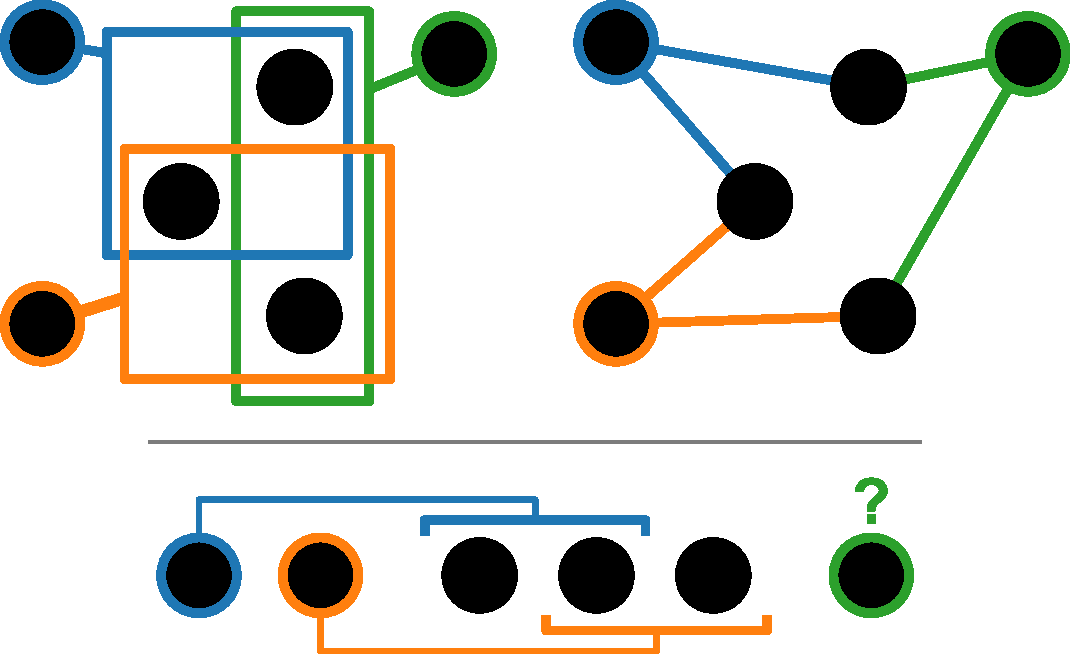
\includegraphics[width=.85\textwidth]{joy/niche.pdf}
  \caption[An illustration of food web dimensionality]{An example of a food web that cannot be one-dimensional, when following the definition in Section~\ref{sec:topology}. Top-left is a two-dimensional niche drawing, where coloured boxes indicate the group of prey for a predator. Top-right is the corresponding node-link diagram.
  The bottom drawing shows why only having one dimension cannot position the prey such that each pair is adjacent.}
  \label{fig:niche}
\end{figure}

It may then seem impossible for the player to effectively explore this search space, but low-dimensional topologies should mean that simple strategies and patterns can be used to successfully construct them.
Fortunately, a study by Eklof et al.\ \cite{Eklof2013} collected a massive amount of data to directly ask the question: what dimensionality do empirical food webs exhibit? Dimensionality in this case is defined as the number of \emph{niche axes} required to capture the topology of a food web, which follows the same definition as the aforementioned niche model. An example of this is shown in Figure~\ref{fig:niche}.

The question was answered by searching for the minimum number of niche axes required to describe the topologies present in the data, by applying an algorithm that searches the space by swapping certain species one by one, and then estimating the `best' dimension using the Akaike information criterion \cite{Eklof2013}. This is necessary because there does not exist a polynomial time algorithm for determining the number of axis required.
Their result was that the number of dimensions needed to describe even the largest webs is surprisingly low. For smaller webs (fewer than 250 interactions) only one dimension was needed, and only four were needed for their best prediction on webs with thousands of species (with a mean of 1.395 over all webs).
This means that simple strategies and patterns should be able to describe any real food web topology, and therefore that humans can hope to form such strategies.

\subsubsection{Trophic levels}
A final topological feature that will be considered is the \emph{trophic level} of each species, specifically the prey-averaged trophic level \cite{Williams2004}, defined as
\begin{equation}
  \mathbf{y}_j = 1 + \sum_i \mathbf{P}_{ji}\mathbf{y}_i
  \label{eq:trophic}
\end{equation}
where $\mathbf{P}_{ji}$ is the proportion of the diet of $j$ that $i$ contributes to.
% I sort of regret only taking constant values for p in the game...
In other words, the trophic level of a species is exactly equal to the mean trophic level of its prey, plus one.
The similarity of this definition to Tutte's algorithm back in Chapter~\ref{chap:stress}, Equation~\eqref{eq:tutte} is worth noting, as the matrix to be solved here is also a graph Laplacian, defined as
\begin{equation}
  \begin{bmatrix}
  1&-\mathbf{P}_{1,2}&\cdots&-\mathbf{P}_{1,n}\\
  -\mathbf{P}_{2,1}&1&\cdots&-\mathbf{P}_{2,n}\\
  \vdots&\vdots&\ddots&\vdots\\
  -\mathbf{P}_{n,1}&-\mathbf{P}_{n,2}&\cdots&1
  \end{bmatrix}
  \begin{bmatrix}
  \mathbf{y}_1\\\mathbf{y}_2\\\vdots\\\mathbf{y}_n
  \end{bmatrix}
  =
  \begin{bmatrix}
  1\\1\\\vdots\\1
  \end{bmatrix}
  \label{eq:trophic_matrix}
\end{equation}
where most of the values of $\mathbf{P}_{ji}$ will be zero because the structure will be reasonably sparse.
The matrix also has the nice property of being diagonally dominant, which means that iterative methods such as Jacobi or Gauss-Seidel are guaranteed to converge~\cite{Young2014}. This will be made use of later in Section~\ref{sec:eco_visualisation}.

It is widely accepted that the trophic level of species has a useful meaning within the context of ecosystems~\cite{Post2002, Johnson2014}. This is because species with high trophic levels tend to be more biologically complex, as they are at the top of the food chain, like humans for example. Trophic level will therefore be made use of in Section~\ref{sec:eco_visualisation} within a visualisation context.

A summary statistic based on the trophic levels of all species is known as \emph{trophic coherence}, and is a measure of how homogeneous the layers of trophic levels are. For example, a perfectly coherent topology would have all integer trophic levels. Specifically, coherence is defined as
\begin{equation}
  \mathrm{coherence}(\mathbf{y}) = \sqrt{ -1 + \frac{1}{|E|}\sum_{\{i,j\}\in E}(\mathbf{y}_i - \mathbf{y}_j)^2}
  \label{eq:coherence}
\end{equation}
and can be interpreted as the standard deviation of differences in trophic level over each edge. It is strictly larger than zero, where zero indicated perfect coherence, and so the larger it is the more incoherent the web.
This quantity was studied by Johnson et al. \cite{Johnson2014}, where it was shown that more coherent topologies result in more stable ecosystems. It will be used here to analyse the strategies taken by players to tackle challenges in the game.

\subsection{Citizen science}
\label{sec:citizen_science}
At the time of writing, the video game industry has grown large enough to eclipse the film and music industries, combined \cite{Egenfeldt-Nielsen2019}. Its recent growth is due to the rise in mobile and competitive gaming, which have rounded out the market to appeal to casual and hardcore audiences respectively.
Their popularity has also spilled into the world of research, with a variety of research-oriented games being produced in a range of disciplines. The motivation behind making such games is twofold, as they can simultaneously perform outreach through public engagement, as well as produce research outcomes through crowdsourcing of human intelligence through player gameplay.

This crowdsourcing is known as \emph{citizen science}, and is not limited to the digital world; it has been successfully applied to physical projects such as measuring soil composition \cite{Rossiter2015}, tracking the global impact of light pollution \cite{Cui2020}, or centralising the work of birdwatching enthusiasts to better track the population trajectories of bird species \cite{Link2008}.
% BES 2019 flower bloom time thing in california?
Even in the digital space, citizen science does not necessarily require a gamified context in order to perform the crowdsourcing. One of the oldest digital citizen science projects is \emph{Galaxy Zoo} \cite{Masters2019}, which tasks players at identifying different types of galaxies from telescope data, in order to build a map of the universe. They have successfully classified the morphologies of galaxies for over a decade, and the data collected has even been used in machine learning contexts \cite{Walmsley2020}.

% The common thread for how. In the context of on problems that computers cannot handle.
The projects most related to the work done here are however the gamified ones. Some of the most successful examples of this include:
\begin{itemize}[leftmargin=*]
  \item \emph{Foldit} \cite{Cooper2010}, a game where the player is given the ablity to fold proteins, with the objective being to find folded configurations with the lowest \emph{Rosetta} energy. This is important because real proteins fold into low energy configurations, and knowing the topology of such states is important to understanding their chemistry. The search space of topologies is too large for computers to currently handle, and so they turn to the spacial reasoning of humans (although Google have recently made attempts at solving this with machine learning \cite{Senior2020}
  \item \emph{Eyewire} \cite{Bae2018}, where players are tasked with analysing pictures of 3D images of brains, collected using an electron microscope. The game aims to leverage the pattern recognition abilities of humans in order to map the exact locations of huge numbers of neurons.
  \item \emph{EteRNA} \cite{Lee2014}, a game conceptually very similar to Foldit, except that it is applied to RNA sequences instead. It is also presented as a 2D interface instead of 3D, which presents a slightly different type of reasoning required to solve its puzzles.
%   \item \emph{BioBlox} 
\end{itemize}

Popular mainstream games have also included citizen science elements within their games. \emph{Borderlands 3}, a game that has sold millions of copies, included a block puzzle similar to Tetris that tasks the player with mapping DNA across gut biomes.\footnote{See \url{www.youtube.com/watch?v=L_mH6Ak_Ny0} for their official promotional explanation.}

The success of these projects shows that the general public has great potential as a scientific resource to be tapped into.
People from non-scientific backgrounds are in general keen to contribute to a scientific cause; Ponti et al.\ \cite{Ponti2018} discuss player motivations and came to the conclusion that participants are driven by scientific ideals such as collaborative progress and democratisation of knowledge. They also warn, however, that introducing too much of a competitive element to the gamification may produce cognitive tension between the two goals of collaboration and rivalry between players.

\subsubsection{Canine inspiration}
\label{sec:yellowstone}
The story behind EcoBuilder is based around historical events in Yellowstone Park, USA. In 1926, wolves were declared officially extinct in the park due to an excess of hunting due to lack of regulation at the time. 
The consequence of this was that elk no longer had any natural predators, leaving them to feed excessively on the park's plants without risk of predation. The resulting supression on plant population had a knock-on effect to smaller mammals such as beavers and fish, causing their populations to struggle, and the health of the entire ecosystem to deteriorate.
This continued until 1995, when ecologists decided to take the action of reintroducing wolves to the park, by capturing fourteen wolves from Canada and transporting them across the border \cite{Smith2003}.

Thankfully, the operation was a success due to the ensuing \emph{trophic cascade:} elk once again had a natural predator, leading to the restoration of plants, bringing back beavers who could again build dams, drawing fish back into rivers, and so on and so forth \cite{Dobson2014}.
EcoBuilder aims to give ordinary people the ability to make similar decisions in their own simulated ecosystems. These simulations will be performed using the equations in Section~\ref{sec:predator_prey}, and so phenomena like the chain reactions seen in Yellowstone can be recreated, as emergent properties of the underlying dynamical system.

The goal, in terms of citizen science, is to create a symbiotic relationship between players and researchers within the context of the game.
Players will learn about how ecosystems function, and why they may fall apart given the wrong structural decisions. In return, players will be tasked with building ecosystems that offer potential solutions to the stability vs.\ complexity debate. A further visualisation experiment will also be performed, with the aim of exploring different types of node layout for food webs. These research outcomes of the game are further discussed in Section~\ref{sec:eco_hypotheses}.
The following section will first study the process behind the design and development of the apparatus where this is made possible.

\section{User interface}
\label{sec:user_interface}
\begin{figure}
    \centering
    \makebox[\textwidth][c]{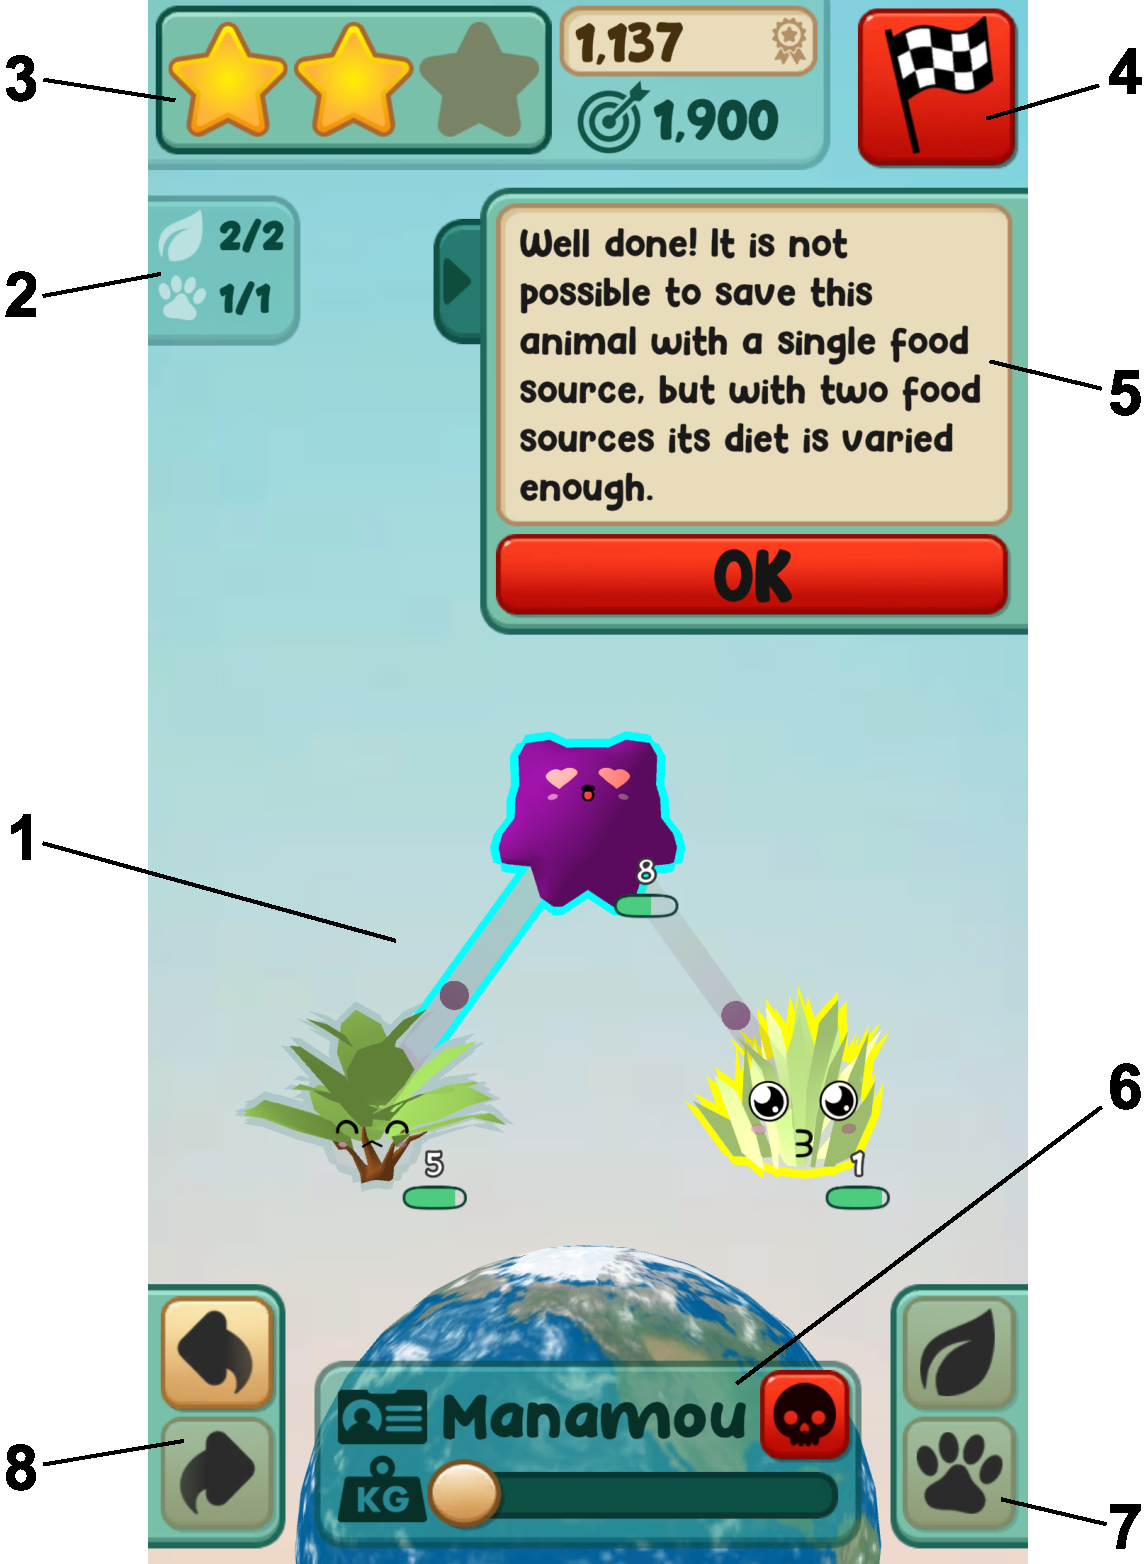
\includegraphics[width=1.09\textwidth]{joy/gameplay.pdf}}
    \caption[A labelled screenshot of EcoBuilder gameplay]{An illustrative screenshot of gameplay in EcoBuilder. The components labelled 1--8 are explained in Section~\ref{sec:user_interface}.}
    \label{fig:eco_gameplay}
\end{figure}

There are multiple components that go into the development of any game, and EcoBuilder is no different. The Unity game engine \cite{Goldstone2009} was chosen as the computational framework, due to its ease of compilation to various platforms, including mobile and WebGL. To illustrate the various engineering challenges behind the user interface, Figure~\ref{fig:eco_gameplay} will be used as a reference screenshot of the gameplay performed by a player. The various moving parts are labelled in the order they will be explained.
However, the best way to gain an understanding of the interface is to try it --- links for downloading the game on iOS and Android can be found at \url{www.ecobuildergame.org}.

\subsection{Food web visualisation}
\label{sec:eco_visualisation}
The most complex component of the gameplay is the visualisation of the ecosystem itself, as it must simultaneously display its topology and dynamical behaviour. For that reason, this whole section will be devoted to its explanation, and the following Section~\ref{sec:HUD} will concern the remaining components.

As shown by label~1 in Figure~\ref{fig:eco_gameplay}, a node-link diagram is used for visualising the topology of the food web.
The nodes of the diagram represent species, where their shape and colour are dependent on the two traits, size and interference (further explained in Section~\ref{sec:HUD}, label~6).
Node colour depends on both traits simultaneously, to span a 2D plane in the 3D CIELAB colour space to maintain perceptual uniformity \cite{Smart2019}, where the planes used for plants and animals can be seen in bottom left of Figures~\ref{fig:101} to~\ref{fig:103}.
Node shapes were designed to be relatively spherical in order to resemble a classical node-link diagram, and change depending on the choice of plant or animal. The cute faces are procedurally generated using random combinations of eyes and mouths.
Links are rendered with low opacity, except with moving circles that flow in the direction of biomass transfer. Such animated edges were studied by Holten et al.\ \cite{Holten2011} to be effective at showing link direction, and also recommended in \cite{Bach2017}.
Coloured outlines around nodes and links are also used to indicate their status, for example in Figure~\ref{fig:eco_gameplay} a blue outline means the component cannot be edited, and a yellow outline means it is the current focus of the panel labelled by the number~6.

To show the equilibrium abundance of each species, as calculated by Equation~\ref{eq:equilibrium}, a small symbol is placed next to each species, which follows the same conventions as battery life indicators on mobile devices, and health bars in video games. Because this abundance can be negative (corresponding to extinction), values below zero are shown as red that only fills a small fraction of the space, and positive values as green that fills up more. An example of negative abundance can be seen in Figure~\ref{fig:ecobuilder_device}.
Numbers showing the exact traits of each species are also placed above the battery icons, so that the exact definition of the species can be exactly identified.

\subsubsection{Interactive layout}
The introduction of interaction adds multiple extra factors that need to be taken into consideration.
The first is the question of how the player adds new edges to the graph. This is done in the simplest and most intuitive manner: the player simply drags in between the two nodes they wish to attach to each other. Since the flow of biomass is directed from prey to predator, the first intuition may be to drag from the prey to predator, however preliminary feedback showed that players found it more intuitive to think in terms of \emph{this eats that}. The default setting in the game therefore has the player drag from predator to prey, but this is left as an option in the settings.

The layout of the nodes is computed by minimising stress, as studied in Chapter~\ref{chap:stress}.
However, an issue is that the topology will change every time the player adds a link, and so the layout must be recomputed each time.
The main problem with this is that stress as an energy function is invariant to rotation, translation, and reflection, so there is no guarantee that any two layouts will line up well at all.
A first attempt to solve this was to use the previous layout as the initialisation for the next. This is effective at maintaining nodes close to each other, but unfortunately can throw the optimisation directly into a local minimum, leading to low-quality layouts. The work in Chapter~\ref{chap:stress} showed that stochastic gradient descent (SGD) does not require smart initialisation to effectively minimise stress, but unfortunately it is not good enough to escape from a bad (i.e.\ worse than random) initialisation.
The game therefore proceeds by reinitialising the layout randomly when the topology of the graph changes, and running SGD from scratch every time. 

The Unity game engine works by providing the programmer with functions to implement that will be run once per frame, but SGD is not quite fast enough to be completely computed every frame and still maintain a good frame rate.
Because of this, the layout code is implemented as a thread that runs concurrently alongside the primary frame-by-frame thread, and only returns the layout to display on the screen once it is completed. SGD is fast enough to only require a couple of frames, even on mobile devices, but threading is still required to prevent stutter.
On top of this, the local version of majorization (see Section~\ref{sec:majorization}) is used once per vertex per frame in order to fine tune the layout slowly into a precise minimum.

However, this brings back the problem of subsequent layouts not lining up well with each other, thus impairing the user's mental map \cite{Eades1991, Diehl2001} of the graph. This problem is known as \emph{dynamic} graph layout in the literature.
A variety of ideas to deal with this problem have been proposed, such as tweaking a force-directed model to minimize Bayesian probability differences between layouts \cite{Brandes1997}, or considering the two graphs at the same time but with additional edges attached between corresponding nodes \cite{Erten2003}. Simplifying the union of the two graphs using a hierarchical decomposition, similarly to those studied in Chapter~\ref{chap:power}, and depicting only the movement of the hierarchy is another creative idea \cite{Archambault2009}. Presenting the user with multiple timeslices of the transition in a grid, rather than through animation, has also been shown to improve task response times, although at the expense of accuracy \cite{Archambault2011}.

Since the changes from subsequent topologies only differ by at most a single edge, and the considered graphs are small i.e.\ fewer than a couple dozen vertices, it was decided that the state-of-the-art methods mentioned above were not necessary for this use case. A simple linear equation to describe the player's mental map is instead used, known as the \emph{Procrustes}\footnote{The name Procrustes is derived from Greek mythology, and translates to `stretcher'. It is based on the story of a man named Damastes, who was given it as a nickname because he would offer unsuspecting travellers a place to stay for the night, but proceed to stretch their limbs on a rack if they did not exactly fit the bed. Karma eventually caught up to Damastes when he experienced the same fate as his guests at the hands of Theseus \cite{Cox2000}.} statistic.
This is simply defined by the sum of squared distances between two layouts
\begin{equation}
  \mathrm{procrustes}(\mathbf{X}, \mathbf{X}^\prime) = \sum_{i\in V} ||\mathbf{X}_i - \mathbf{X}_i^\prime||^2
  \label{eq:procrustes}
\end{equation}
and can be exactly minimised using linear transformations.
% The square root of the right-hand side is usually taken as the final value
Removing the translational component is performed by simply placing the barycenter of both layouts at the origin. Traditionally $\mathbf{X}'$ is then dilated, but stress is not invariant to scaling so this step is skipped here. The rotational component is then removed by differentiating the right-hand side of Equation~\eqref{eq:procrustes} with respect to a rotation $\theta$ and solving for the derivative equalling zero, resulting in
\begin{equation}
  \theta(\mathbf{x},\mathbf{y}, \mathbf{x^\prime}, \mathbf{y^\prime}) = 
  \tan^{\text{--}1}\left(\frac{\sum_i(\mathbf{y}_i\mathbf{x}^\prime_i-\mathbf{x}_i\mathbf{y}^\prime_i)}{\sum_i(\mathbf{x}_i\mathbf{x}^\prime_i-\mathbf{y}_i\mathbf{y}^\prime_i)}\right)
\end{equation}
where $\mathbf{x}$ and $\mathbf{y}$ are the two dimensions of the layout $\mathbf{X}$, and similarly for $\mathbf{X}^\prime$. Since the dilation step was skipped, this process is performed for both the new layout and its reflection, where the result with a lower value of Equation~\eqref{eq:procrustes} is chosen. Note that usually in the literature, the square root of this value is taken as the final statistic.

This definition has been previously used to assess the similarity of layouts given any linear transformation \cite{Ortmann2017}, and is used in the game in order to align subsequent layouts. If the sets of vertices differ between topologies, then their union is instead compared.
To transition smoothly between aligned layouts, the \texttt{SmoothDamp()} function provided by Unity is used, which attaches a critically damped spring between an object and its target position, to avoid jerky movement by maintaining continuity \cite{Kirmse2004}.

\subsubsection{Constraining the y-axis}
A domain-specific feature of food webs is that any valid topology allows for the trophic level to be calculated for each species, following the process outlined in Section~\ref{sec:topology}. For this reason, an additional constraint to the layout is included, that constrains the y-axis to the trophic level of the species.

The diagonal dominance of the Laplacian matrix to be inverted in order to solve for trophic levels allows for the Jacobi method to be used. Expressing the trophic level Equation~\eqref{eq:trophic_matrix} as 
\begin{equation}
  \mathbf{y} = \mathbf{L}^{\text{--}1}\mathbf{b},
  \label{eq:trophic_laplacian}
\end{equation}
ordinary Jacobi solves for $\mathbf{y}$ by assigning
\begin{equation}
  \mathbf{y}_i^\prime = \frac{1}{\mathbf{L}_{ii}}\left(\mathbf{b}_i - \sum_{j\neq i}\mathbf{L}_{ij}\mathbf{y}_i\right)
\end{equation}
for each vertex $i$ \cite{Young2014}. In this case, $\mathbf{b}$ is simply a column vector of ones.
An iterative method was chosen because the topology of the graph will only change by a single edge at a time, and so previously calculated trophic levels is a good approximation for subsequent values. From experience, the number of iterations required for convergence is almost always fewer than ten. Since the matrix $\mathbf{L}$ contains an entry for every edge, the complexity per iteration is $\mathcal{O}(|E|)$, as opposed to solving the system exactly. 
Equation~\eqref{eq:trophic_laplacian} does not have a solution if any component has no vertex with an in-degree of zero (i.e.\ no primary producers). In this case, trophic level computations are simply ignored.

% 3D vs 2D: originally used 3D, but we found that players could not quickly pick up the rotational interface. Nodes would also often become obscured in the center of the layout, so we switched to 2D instead. 
A problem here is that stress is more difficult to optimise, because there is now only one degree of freedom for vertices to move around in. The solution found was to increase the maximum value of $\mu$ in Equation~\eqref{eq:mu} to $1.1$, as well as adding five extra initialisation iterations at the beginning of the optimisation. This is however an ad hoc solution and future work should involve testing variations of this systematically.
The aforementioned Procrustes statistic also skips the rotation step in this case, as any rotation would break the orientation of these constraints.

An important question is whether constraining the y-axis is helpful to the user in the first place. Intuition says the constraint will largely make edges point upwards, which should help to preserve the player's mental map of the flow of biomass throughout the system. The opposing argument is that layouts will have higher stress, and so may become more crowded.
This question will be systematically tested by the game. Half of the players will be given an standard layout and the other half a constrained layout, and data collected from the game will be used to study which is more effective. More detail on this experiment is outlined in Section~\ref{sec:eco_hypotheses}.

\subsection{Heads-up display}
\label{sec:HUD}
The remaining labels on Figure~\ref{fig:eco_gameplay} point to elements of a 2D overlay, upon which exists what is known as a heads-up display (HUD). The idea of a HUD is now ubiquitous to video game interfaces, but its name originated from military aviation, where the pilot would need to have extra information available whilst leaving their view unobstructed. 
Its purpose in the context of games is the same, where it gives the player the remaining information required to complete the game, whilst leaving the main visualisation as visible as possible.

\subsubsection{Label 2: Constraints}
Different levels offer different scenarios, with specific topological constraints shown on this first panel. The top two icons show the maximum numbers of plants and animals the player may introduce, and the bottom two show the number of edges and the maximum chain length. Chain length is defined for each plant as zero, and each animal as the shortest path from any plant to it. These are all used throughout the game as conditions required to pass each level.

Earlier versions of the game also included maximum loop length as an extra constraint, but there does not exist a polynomial time algorithm to search for all loops in a graph. Johnson's algorithm \cite{Johnson1975} was attempted for this, but its running time grew unacceptable and so it was cut from the final release of the game.

\subsubsection{Label 3: Score}
This panel displays the player's score, as well as how many stars they have obtained. To obtain the first star, the only conditions are that all species coexist and that there is a single connected component. The second and third stars require the player to reach certain numerical score thresholds as a further challenge for skilled players. The current score is shown as the number in the pale brown sub-panel, and the target is shown as the green number below.

Many different metrics were tried and tested for use as a score, most of which were unsuitable. For example, the total abundance every species was a good candidate, but this is maximised by having only plants in the food web, as any animals simply lose too much biomass via the efficiency factor $e_0$ in Equation~\eqref{eq:interaction_strength}. The score should instead continuously increase as the food web becomes more complex. Another related option was to take the total \emph{flux} of the food web, defined as the total amount of biomass flow through every interaction. This is defined here as the sum of the positive off-diagonals in Equation~\eqref{eq:jacobian_evaluated}.

One definition of quantitative complexity is $\sigma\sqrt{nC}$, where $\sigma$ is the standard deviation of the off-diagonals of the community matrix in Equation~\ref{eq:jacobian_evaluated}, $n$ is the number of species, and $C$ is the connectance, defined as the proportion of realised to possible interactions such that $0\leq C\leq1$. Specifically this is $C=|E| / (n(n-1)/2)$. This quantity was shown by May to negatively correlate with the probability of stability as defined in Equation~\eqref{eq:lambda_stability}, and acted as the springboard for the aforementioned complexity vs.\ stability debate.
This criterion has been taken and updated to more accurately match real ecosystem structure \cite{Allesina2012, Tang2014Correlation}, but all contain the components $\sigma$, $n$, and $C$.
Unfortunately none of these metrics were able to fit the purposes of a game, because the factor $\sigma$ is not very interpretable, and players found it difficult to work out why it would go up or down.
% sometimes super suddenly. It was also maxed out at 2 species
Leaving out $\sigma$ and only including $n$ and $C$ does not work either, since they are both structural measures and so do not capture any dynamics of the system.

The final formulation settled upon was a compromise between the aforementioned options: the factor $\sigma$ is replaced by the total abundance and the square root removed, to construct a final score of
\begin{equation}
  \mathrm{score} = \left(\sum^n_i\mathbf{z}^*_i\right)nC
  \label{eq:score}
\end{equation}
where $\mathbf{z^*}$ is from Equation~\eqref{eq:equilibrium}. This alternative is interpretable and goes up as the food web grows in size.
Unfortunately, this leaves us with a metric that does not have any direct significance in terms of answering a research problem, so is not suitable for crowdsourcing the answer to an ecological question. This problem will be discussed in Section~\ref{sec:research_world}, where the player will be given two alternate scoring metrics that are of interest.

\subsubsection{Label 4: Level}
The square in the top right of the HUD is a button that represents the level currently being played. When the player has earned the first star of a level, this button can be pressed to pass the level and unlock the next. The appearance of this button before the level has been passed can be seen in Figure~\ref{fig:ecobuilder_device}, where pressing it gives the option to quit the game or reset the level. The screen shown to the player upon completing a level is shown in Figure~\ref{fig:eco_server}, left.

\subsubsection{Label 5: Help}
This panel is present throughout the game, in both menu screens and during a level playthrough. It was necessary to not overfill this box for two reasons: the first is that the target platform for the game is mobile devices, so space is limited; the second is that in preliminary playtests, players tended to skip any long blocks of text. Some players would even skip all text, regardless of length, and so care had to be taken to use a `learn-by-doing' approach as often as possible. For that reason, multiple levels that act as heavily guided and constrained tutorials were included.

The green arrow on the edge of the panel can be used to hide or show the text at will.
If the player does not find the solution to a level after two minutes, the text also shows itself to reveal a hint. Further playtests showed that the sometimes counter-intuitive behaviour of the simulation can be frustrating to players, so giving extra help after a delay was a necessary step, a technique often used by game developers to ensure that players get stuck as rarely as possible.

\subsubsection{Label 6: Inspector}
This panel is known as the inspector, and is the avenue through which the player views and changes the traits of their species.
These two traits, body mass and interference, take a wide range of values: mass goes from one gram to one thousand kilograms, therefore spanning six orders of magnitude; interference goes from 10$^{\text{--}4}$ to 10$^{\text{--}1}$, spanning three orders of magnitude. This range for mass was chosen to capture species of almost all sizes in the natural world. Smaller species do exist and are vital to Earth's ecosystem (such as bacteria and the smallest insects) but they are left as out of scope for the game.
The range of interference values was set to span this range, as preliminary playtests showed that species with any larger interference tended to be very difficult to keep alive at all, and species with any smaller interference tended to destabilise the rest of the food web.
Preliminary tests also showed that allowing the player to choose interference on top of body mass was too much information for players to begin with. The ability to tweak interference by hand is therefore not unlocked until the second set of levels known as Research World is reached (see Section~\ref{sec:eco_hypotheses}).
Further discussion of interference values can be found in Section~\ref{sec:hypothesis2}.
% The range of interference values is set to span the range of values that the off-diagonals of the interaction matrix can possibly take when parameterised with Equation~\ref{eq:interaction_strength}, using the aforementioned range of body masses. This was done because it is not known what range of values interference takes in nature, and so the assumption was taken that it should not differ too greatly from the magnitude of inter-species interactions.
% interference goes from 1e-5 to 1 (reference hsi-cheng's work)

Both traits are also set according to a log scale, so that all orders of magnitude are accessible. The sliders themselves are constrained to only take discrete values, so that the player knows the exact values being used. This also means that values can be displayed using a single number next to the species, as shown in the screenshot in Figure~\ref{fig:eco_gameplay}.

The button to the upper-left of the panel can be used to remove unwanted species from the food web. It is placed next to the name of the species, which is randomly generated by joining together sequences of syllables.\footnote{Credit for the random name generation algorithm goes to \url{www.fantasynamegenerators.com}, accessed 13/8/20.}
The player may also input their own name for each species, if they wish to do so.

\subsubsection{Label 7: Initiator}
This panel contains two buttons that are used to initiate the addition of a new species to their ecosystem.
It is at this point at which the binary choice between plant and animal is chosen and fixed, which not only makes sense from a biological standpoint, but is also necessary in terms of topology, because plants must have an in-degree of zero i.e.\ they cannot be predators. This is not strictly true for the real world, because species such as the Venus flytrap are in fact carnivorous plants. There are even animals that can perform photosyntesis, such as the sea slug, which can `steal' the ability to produce chloroplasts from the algae it eats \cite{Rumpho2008}.
These such creatures, as remarkable as they are, were considered rare enough to leave out of scope for EcoBuilder.

At this point it is worth mentioning that the number of plants was also limited to a maximum of three in any given level, and usually fewer. This was necessary here because there is no explicit competition between plants, i.e.\ a $(-,-)$ pair in the interaction matrix, and so there is no penalty at all for adding more of them.
This decision was made because of the difficulty behind parameterising these extra interactions, and so the limiting of the number of plants was instead used. Other plant growth models such as the \emph{chemostat} model \cite{Sommer1983} were also considered, but not utilised in the final version.

\subsubsection{Label 8: Recorder}
The final component of the gameplay in EcoBuilder is that ability to undo and redo actions, a feature now considered standard among most consumer applications. The arrow pointing left goes backward to undo an action, and the arrow pointing right goes forward to redo a previously undone action, as is conventional. It is implemented simply using a stack, and so undone actions are lost forever if a new action is performed.
The criteria for being an action is a topological change, i.e.\ the addition or removal of vertices or edges, or a change in value for the trait of a species.

The entire sequence of actions performed by the player is recorded, and when the level is completed it is transformed into a string to sent to a server, along with other playthrough data. The remaining contents of this data will be explained in the following section.

\subsection{Data collection}

\begin{figure}
    \centering
    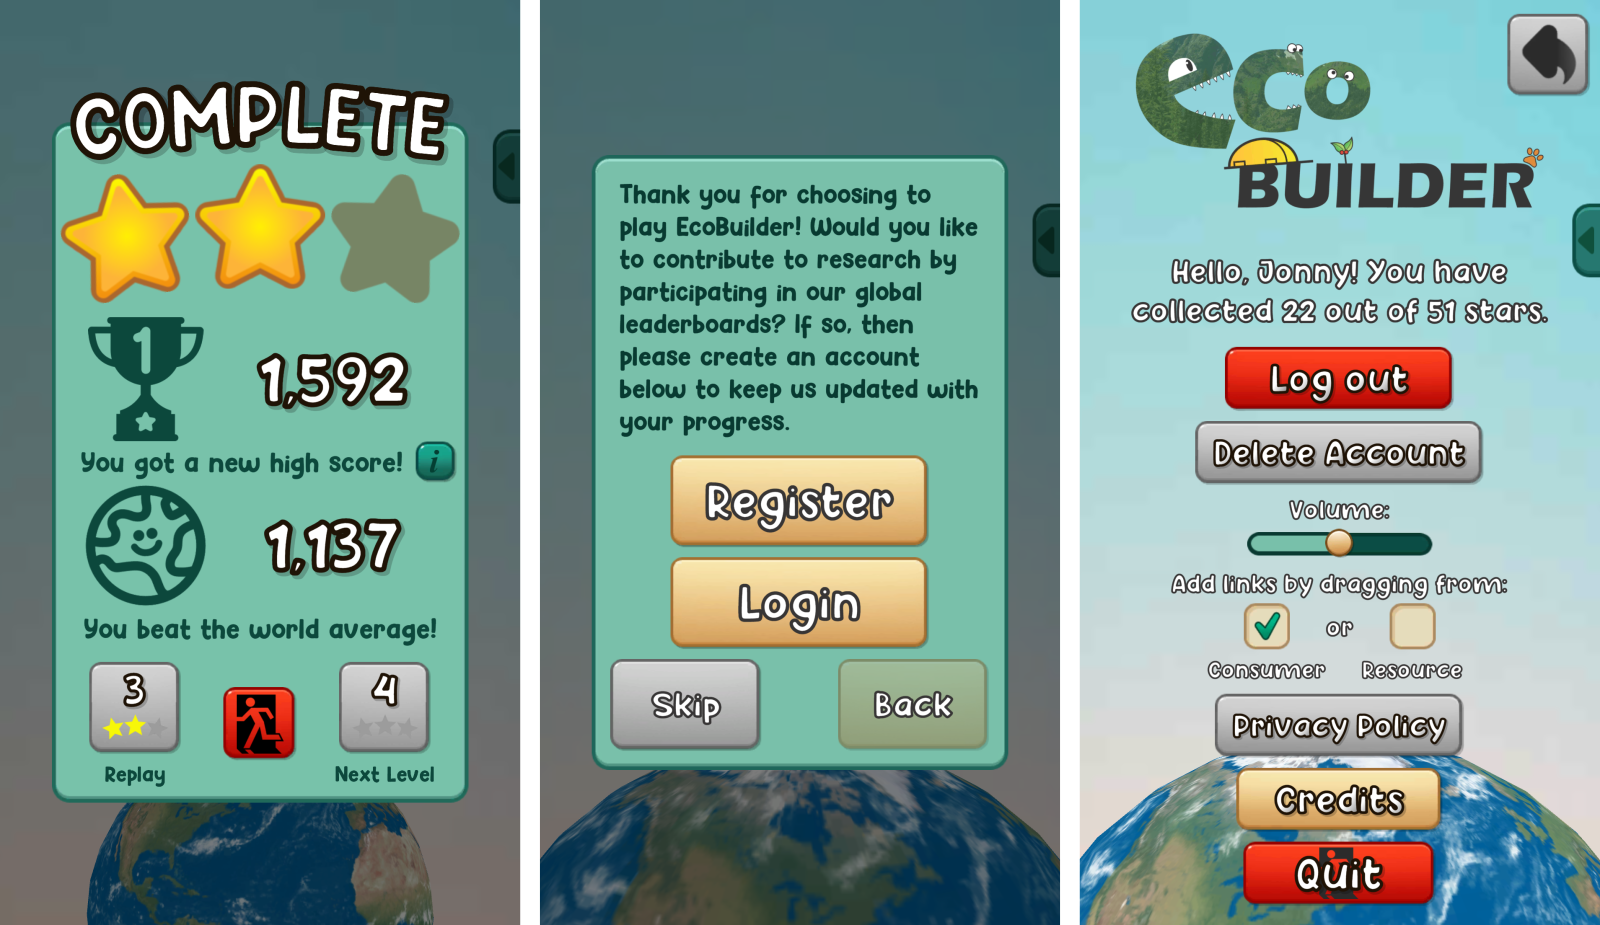
\includegraphics[width=\textwidth]{joy/server.png}
    \caption[Player registration and data collection]{Screenshots to illustrate player registration and data collection. From left to right: the report screen shown when a level is completed, the registration page for player accounts, and the settings page for account details.}
    \label{fig:eco_server}
\end{figure}

Figure~\ref{fig:eco_server}, left, depicts the report card shown to the player when they complete a level. It tells the player the number of stars they achieved, their score, and the median score from all high scores throughout the world. The median score is shown in order to motivate the player to strive for higher scores, as a small competitive incentive.
The small button to the middle-right of the panel can also be pressed to show the exact decomposition of their score, as defined by Equation~\ref{eq:score}, but scaled to fall within a reasonable range of values that make sense as a score. The player can then replay the level or continue to the next.

When this report card panel is shown, a POST request is sent to the server containing multiple fields, including: a timestamp, the score, each component of the parameterisation defined by Equation~\ref{eq:interaction_matrix}, a list of timed actions performed by the player, and a list of device metadata such as operating system and resolution.
These fields are received by the server and stored in an SQL database for future analysis.

The middle screenshot in Figure~\ref{fig:eco_server} shows the registration page that is shown the first time the application is opened. An account is required for two purposes: the first is to ensure that the data being collected can be matched to a single player, even if they decide to switch devices; the second is to have them tick a box to indicate that they are aware of the general data protection regulation (GDPR) their data will be held under. Note that since there is no `sensitive' personal data being collected, such as ethnicity or political opinions, a tick box is not strictly necessary.
Some general demographic information, such as age and education background, is optionally collected at registration.
The player may also delete their account whenever they wish, as shown by the settings page to the right of Figure~\ref{fig:eco_server}. Here they may also change game settings such as volume or drag direction. They may also view the GDPR privacy policy in full, and a credits page to thank the lab members who kindly gave their time to help playtest the game.


\section{Experimental design}
\label{sec:eco_hypotheses}
The gameplay of EcoBuilder is split into two sets of levels. The first set is called `Learning World', and the second is `Research World'. 
When the player first opens the game, they are greeted with two large buttons that lead to the two Worlds. Initially, Research World is locked and may only be entered when they complete all the levels in Learning World, as shown in Figure~\ref{fig:eco_worlds}, left. This gives the player an incentive to complete the Learning levels, and also ensures that all players have received the same introduction before tackling the more difficult problems presented in the Research levels.

\subsection{Learning World}
\label{sec:learning_world}
Learning World contains 18 levels in total, all of which contain relatively simple scenarios designed to be instructive. For example, levels 3 and 4 both force the use of a heavy animal that cannot be saved with a single plant, to teach the player that heavier species consume slower (on a mass-specific basis) and so require more abundant food sources. Levels 5 and 6 present the player with a situation known as \emph{competitive exclusion}, a well-known natural phenomenon that states that if two predators share the exact same prey, then the predator with a faster intake rate will almost always drive the slower to extinction.
The real-world example of this told to the player is the exclusion of red squirrels after the introduction of grey squirrels in Britain, due to their superior foraging ability \cite{Gurnell2004}.
This principle, although predicted by the mathematical model, is however not as common in nature as one would think. Examples such as the `paradox of the plankton' seemingly ignore the principle entirely, as tens or hundreds of plankton species are able to coexist despite sharing the same resources \cite{Hutchinson1961}; results from the game may help to reveal why this occurs.

\begin{figure}
    \centering
    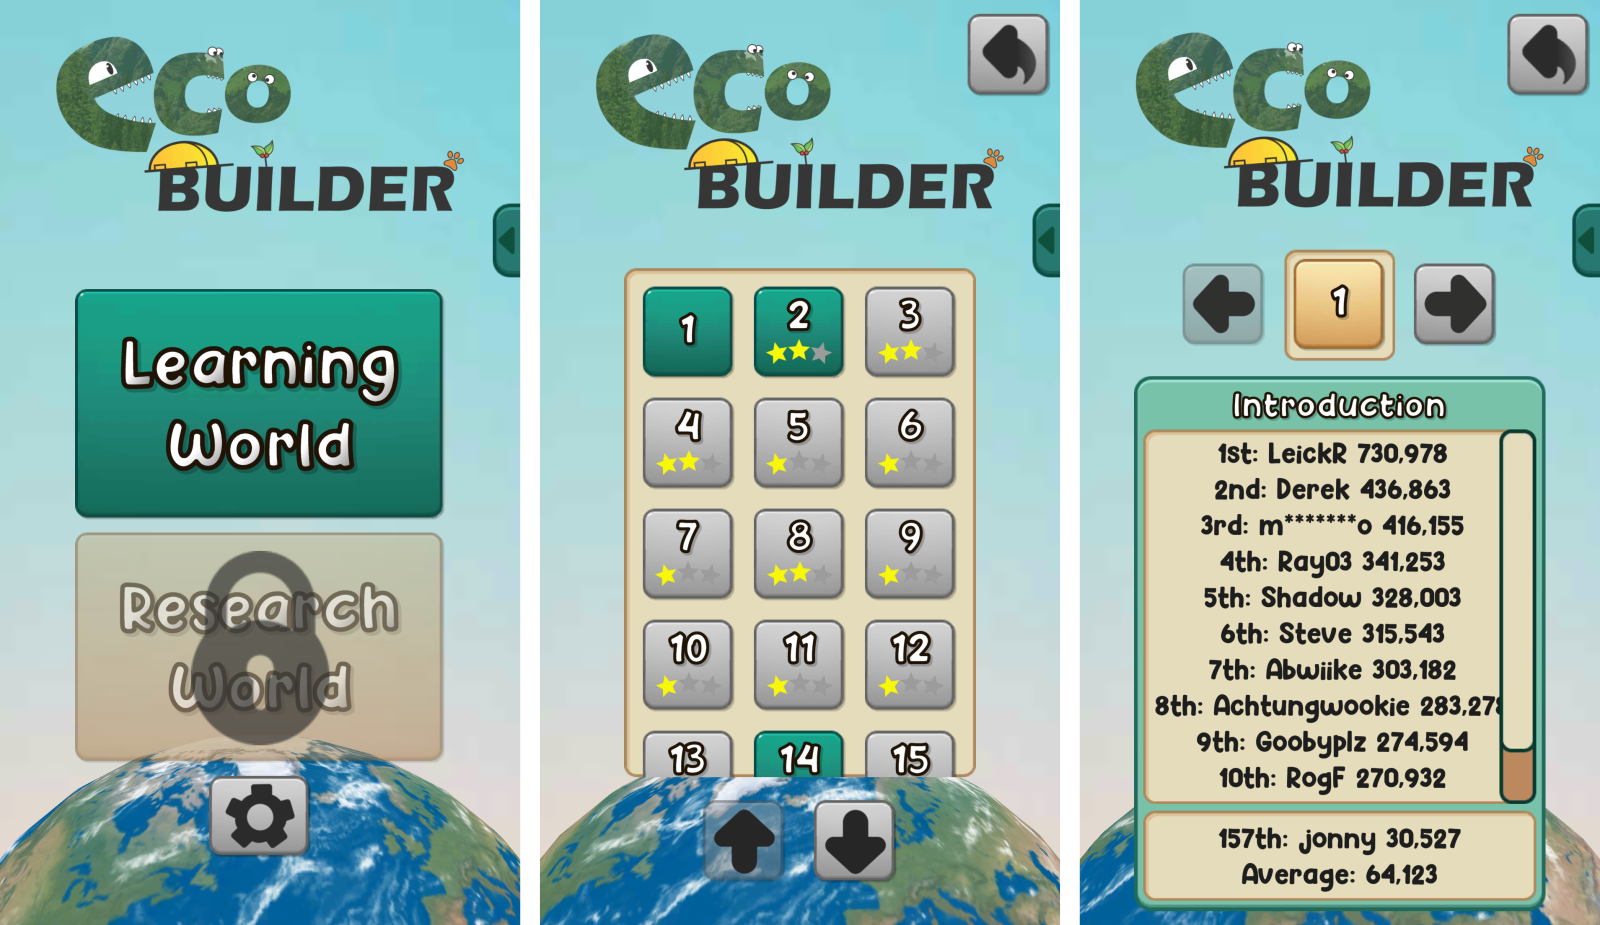
\includegraphics[width=\textwidth]{joy/worlds.png}
    \caption[Learning World and Research World]{Screenshots to illustrate Learning and Research World. From left to right: the splash screen the user sees when they start the game, the list of levels in Learning World, and the leaderboards in Research World.}
    \label{fig:eco_worlds}
\end{figure}


EcoBuilder is a \emph{puzzle} game, in that the player is not tasked with time constraints or tests of dexterity. It is therefore a direct test of the ability of the player to understand the dynamics of the underlying simulation.
This presents the opportunity to perform a controlled test to measure the extent of this understanding. In this case, two node layout methods will be tested, where is computed by simply minimizing stress, and the other additionally has the y-axis positions of species constrained to their trophic level. The layout with only stress optimised will be referred to as the \emph{standard} layout, and with y-axis constrained as the \emph{trophic} layout.
Other experiments in the literature generally give participants topological tasks such as finding paths between nodes \cite{Bach2017, Okoe2018} or deciding which nodes would disconnect the network if removed \cite{Purchase1997}. A novel difference with the experiment here is that there is an actual dynamical system for the participant to further understand.

\subsection{Research World}
\label{sec:research_world}
Research world contains 3 further levels for the player to play, each with a different scoring metric. These levels act more like a \emph{sandbox}, where players may add up to 48 species (limited due to the uniqueness constraint explained below) in whatever topology they wish.
They are given a single task: get as high a score as possible. This score in level 1 is simple the same as in Learning World, i.e.\ Equation~\ref{eq:score}. Level 2 adds an extra one million points per each additional animal, which is so large that it effectively means that Equation~\ref{eq:score} is only included as a tie-breaker. 
Level 3 also gives blocks of a million points, but for each additional max chain length instead of each animal.
To incentivise players to reach for high scores, each of these three levels has a leaderboard for skilled players to aim to be the best, as shown in Figure~\ref{fig:eco_worlds}, right.
The purpose of Research World is to see how players approach these three situations, all of which do not have an immediately obvious solution.

There are a couple of extra details that first must be addressed, however, before letting players loose. The first issue is that there are many trivial solutions if the player is allowed to add many identical species. This is because the main cause of extinctions in the simulation is due to chain reactions such as the aforementioned competitive exclusion, but these do not occur if species are identical \cite{Armstrong1980}. For this reason, no two species are allowed to have the same set of traits. Since there are 9 possible values for body mass and 5 for interference, this results in an upper limit of 45 combinations, plus the binary choice of plant or animal. The number of plants is limited to 3, leaving a total of 48 species per web: more than enough to comfortably fill the screen of a mobile device.

The final addition to Research world is another tool for navigating the topology of food webs. If a species is tapped twice, the layout transitions into a mode where only the direct connections to that species are visible, where its prey are positioned below it and its predators above. The topology can then be navigated in this mode, by hopping from one node to another by again tapping.
This extra feature was necessary because as the number of species goes up, layouts can become crowded and difficult such that it is difficult to see fine details. The extra layer of interaction helps to alleviate this.
% Unfortunately, minimising stress is not able to prevent the problem of crowded layouts. This situation can happen easily for topologies with many edges, and leads to nodes being bunched up closely together. superfocus was our eventual solution, but we do the learning world controlled test without.

\subsection{Hypotheses}
With these details in mind, it is possible to state two hypotheses:
\begin{mdframed}[backgroundcolor=WhiteSmoke]
  \begin{itemize}[leftmargin=*]
    \item \textbf{Hypothesis 1:} Trophic level layout constraints will help players to complete Learning World faster.
    \item \textbf{Hypothesis 2:} Players will be able to successfully find strategies to achieve high scores in Research World, but most will not.
    \end{itemize}
\end{mdframed}
The reason behind the first hypothesis is because constraining species to their trophic level tends to orient edges upwards, which should help to preserve the player's mental map of the flow of biomass through the system. However this does remove a degree of freedom from the optimisation of stress, and so layouts may become more difficult to read for more dense topologies, thus hindering the player instead.

The second statement is slightly vague on purpose, because it is not known what is meant by a `high' score, before letting players try it themselves.
The reason for predicting that most will not find success is because the dynamical systems involved are complex and sometimes counterintuitive, and expecting all players to gain a good intuition for what strategies work well is unrealistic.
The evaluation of this second hypothesis in general will therefore involve more exploratory and speculative analysis than the first.

\section{Results and analysis}
\label{sec:eco_results}

Data from a total of the 842 players who completed at least one level, and over 9000 individual playthroughs were analysed to produce the results presented here. The analysis will begin with examining player performance in Learning World, and then finish with Research World.

\subsection{Hypothesis 1}
\label{sec:hypothesis1}
Hypothesis 1 concerns the performance of players as they progressed through Learning World, depending on the type of visualisation they were presented with, as detailed in Section~\ref{sec:learning_world}.
The first question to ask is: how many levels did players complete before stopping? This is answered in Figure~\ref{fig:player_progression}, where bar charts containing the furthest level reached and number of stars collected can be seen.
\begin{figure}
    \centering
    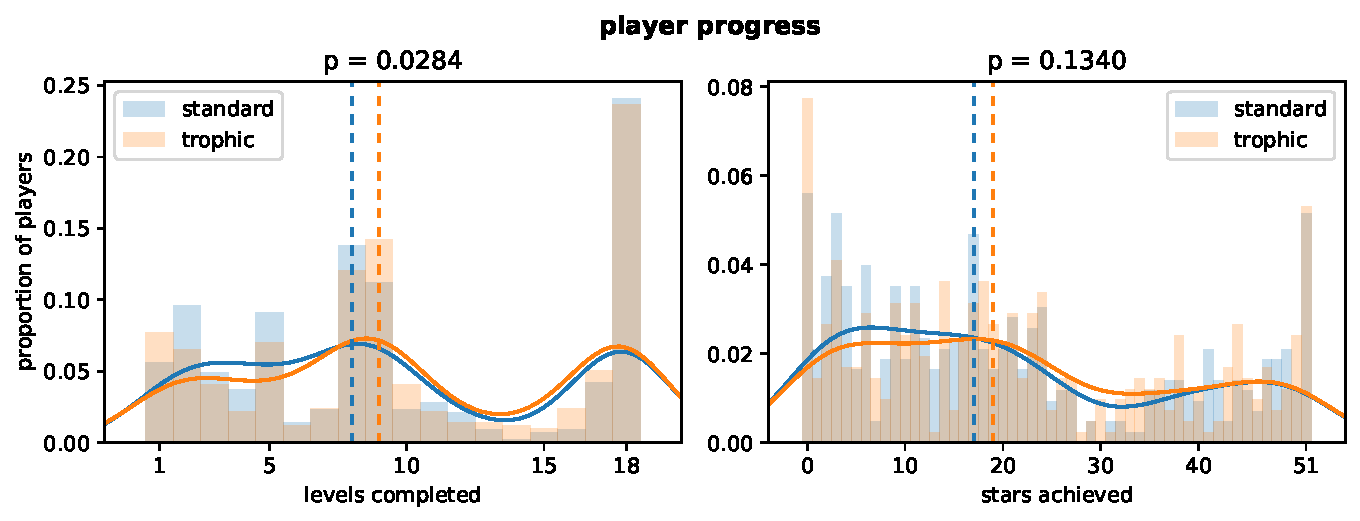
\includegraphics[width=\textwidth]{joy/stars.pdf}
    \caption[Bar charts showing player progressed]{Bar charts showing how far players progressed through the game, for both the standard stress layout and trophically constrained groups. On the left is how many levels were completed, and on the right is how many stars were collected. The smooth curves denote a kernel density function over all bins, and the dotted vertical lines mark the median. The p-value of the trophic median being larger than the standard is written above each plot.}
    \label{fig:player_progression}
\end{figure}
The test statistic studied here for both plots is the \emph{median}, marked by vertical dotted lines for both plots, where it can be seen that progress is slightly further for the trophic group for both measures.
To validate the significance of this result, a permutation test was performed with the null hypothesis that there is no difference in medians between the two layouts is zero.
This was done on 100,000 permutations of the test set, and the resulting p-values are written on top of the corresponding charts in Figure~\ref{fig:player_progression}.

The p-value of 0.028 for levels completed provides a clear yes to the question of which group made it further through the game. The corresponding result for number of stars achieved is not as convincing, but is still positive nonetheless.
Looking at the shape of levels completed, there is a big cutoff at levels 8 and 9, which is a sign that those two levels where designed to be a little too difficult. However, almost all players with the perseverance to make it over that hump continued on to complete the remaining levels. This was the biggest group of players in general, coming in at just under 25\% of all players.

However, this difference in progress through levels makes it incorrect to directly test hypothesis 1 by simply looking at the total play time of players, since playing more levels will increase total play time. A look at the data indeed confirms that the median play time of trophic players was longer.
Because of this, the time element will be analysed on a level-by-level basis. This can be seen in Figure~\ref{fig:level_times}, where a histogram of the time taken by both sets of players is plotted for each of the 18 levels in Learning World, including p-values over the median for each, as in Figure~\ref{fig:player_progression}.

\begin{figure}
    \centering
    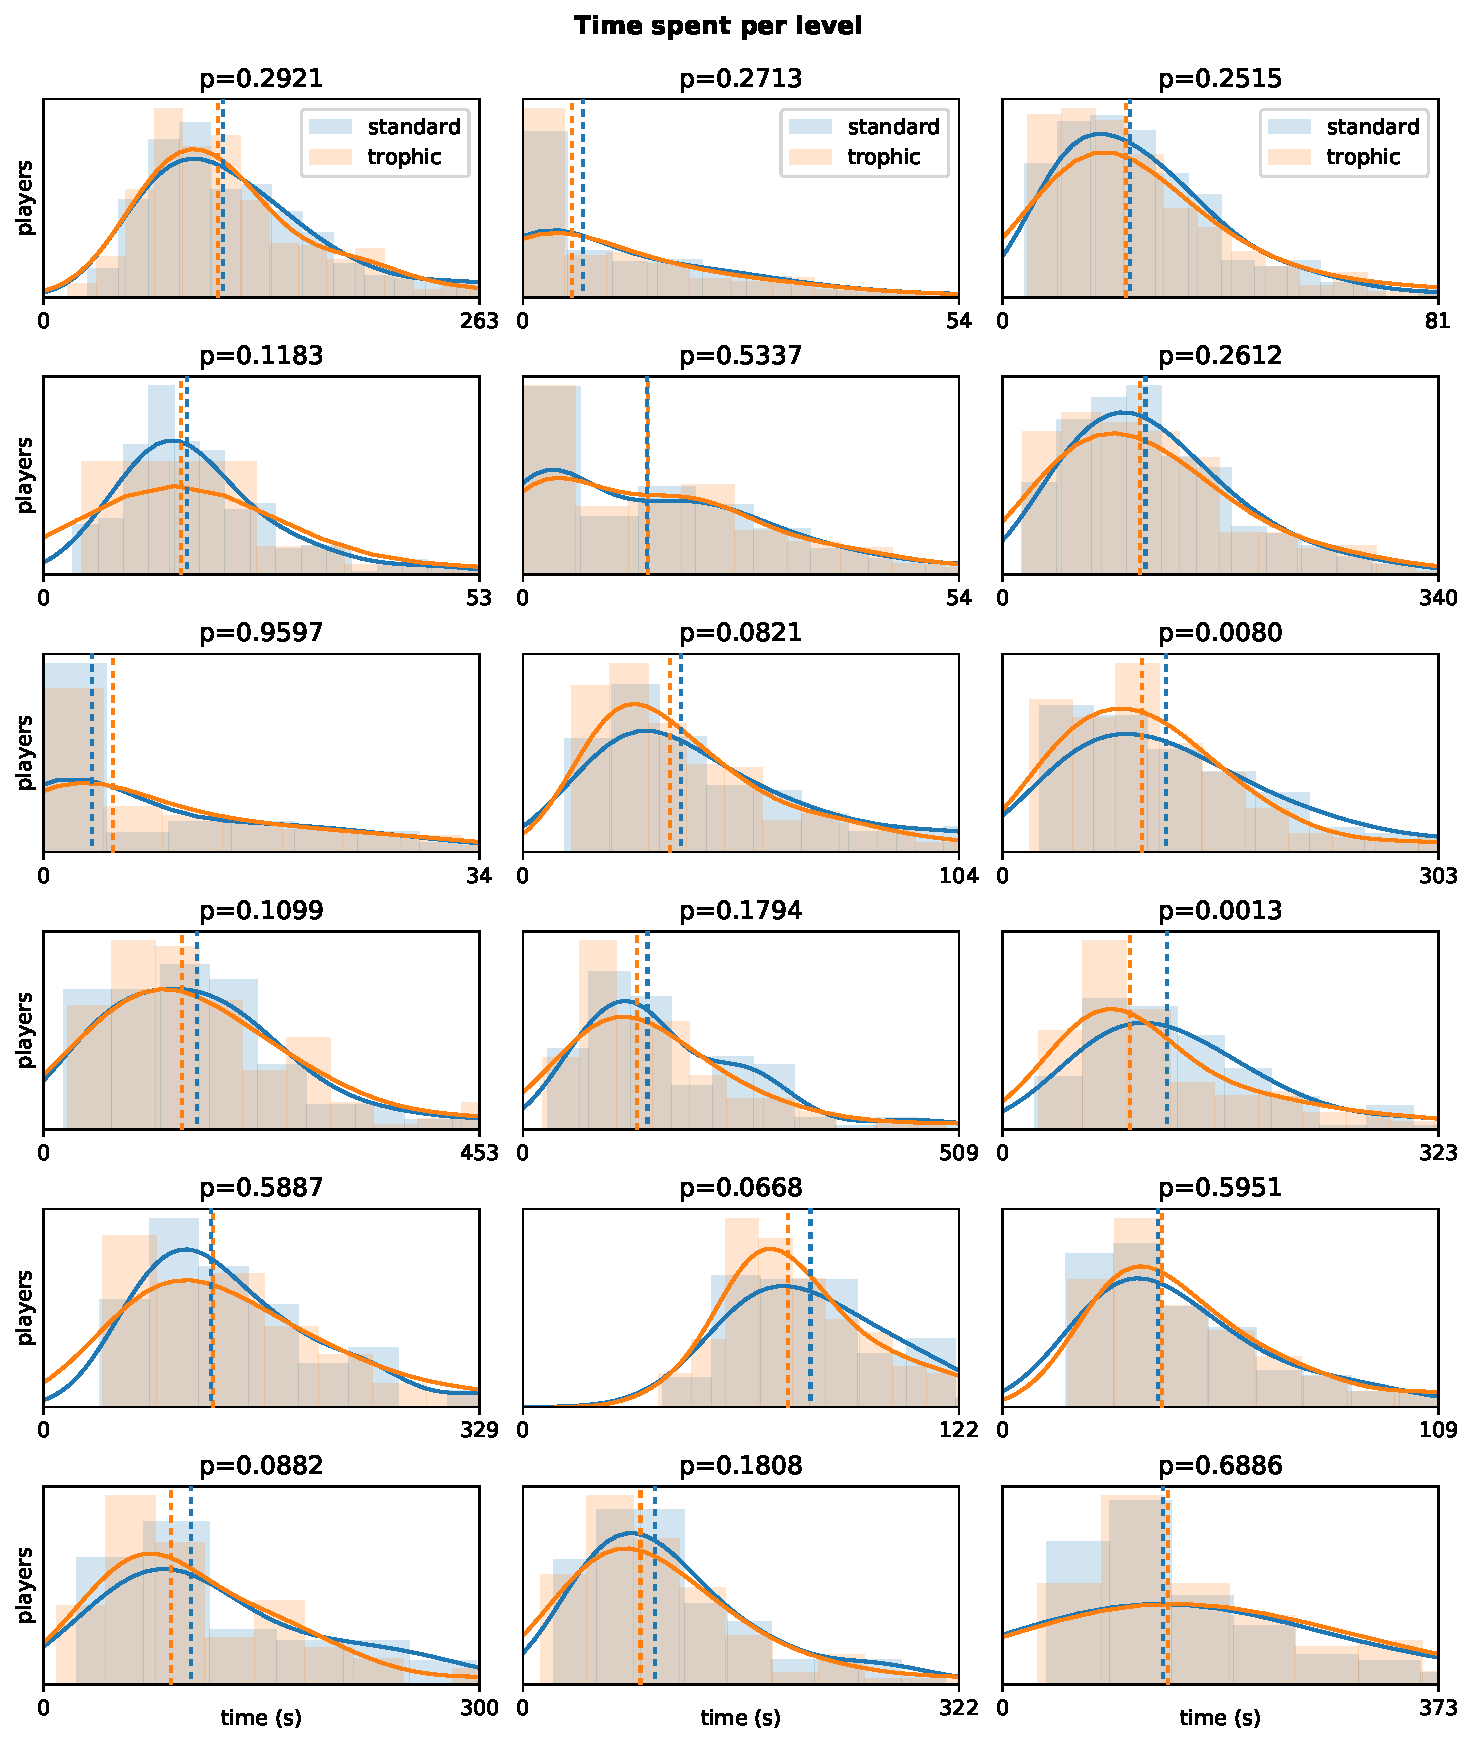
\includegraphics[width=\textwidth]{joy/times.pdf}
    \caption[Histograms showing the time spent on each level]{Histograms of the time taken by both sets of players for every level, with the same conventions as Figure~\ref{fig:player_progression}. The index of each level is written on the top left of every plot, where the upper limit of the x-axis is set to the time at which 95\% of players managed to finish.}
    \label{fig:level_times}
\end{figure}

Not many of the resulting medians are statistically significant, if defined by p-values below 5\%. However, almost every level has a better median for trophic than standard, with many of the more difficult later levels falling below a 10\% threshold.
% The levels that it does do very well on are levels where there more than one trophic level is required.
Level 7 is the only level where the opposite case occurs, and the standard group performed consistently better. However it is also the level that players had the least trouble with in general, with the fastest completion time over all levels.
These results do not mean a shining recommendation for trophic in all situations, but it does show small and consistent improvement over the tasks set for the player.

A peek into research world confirms the need for care when picking a visualisation, as the standard group achieved higher median scores than trophic on the first Research Level, with a p-value of 0.096. This first level simply reuses the score metric in Equation~\eqref{eq:score} which takes connectance into account, and so food webs are naturally going to become especially crowded there. In these situations, fixing the y-axis causes nodes to bunch too closely together to differentiate. Standard layouts still become hairballs, but at least nodes are separated enough to not overlap too much.
Additionally, the remaining research world levels had little to no difference in median scores, which shows that for many tasks there is no value to be gained for adding the trophic constraint to the layout.

These results point towards a small, but clear improvement in performance for the trophic visualisation over the standard one. This is enough to recommend the method for the general application of food webs, but with the condition that care must still be taken to consider the specific use case, as it is not always going to help.

\subsection{Hypothesis 2}
\label{sec:hypothesis2}

After completing Learning World, players unlock the right to compete against each other on three extra levels, as detailed in Section~\ref{sec:research_world}.
The analysis of these levels will be more qualitative than in Learning World, but nevertheless, all three sets of results reveal interesting patterns of how players approached solving the challenges, and of which strategies were good enough to be the very best.

Each level gets its own page of plots, where levels 1, 2, and 3 can be found in Figures~\ref{fig:101}, \ref{fig:102}, and \ref{fig:103} respectively.
\begin{figure}
  \centering
  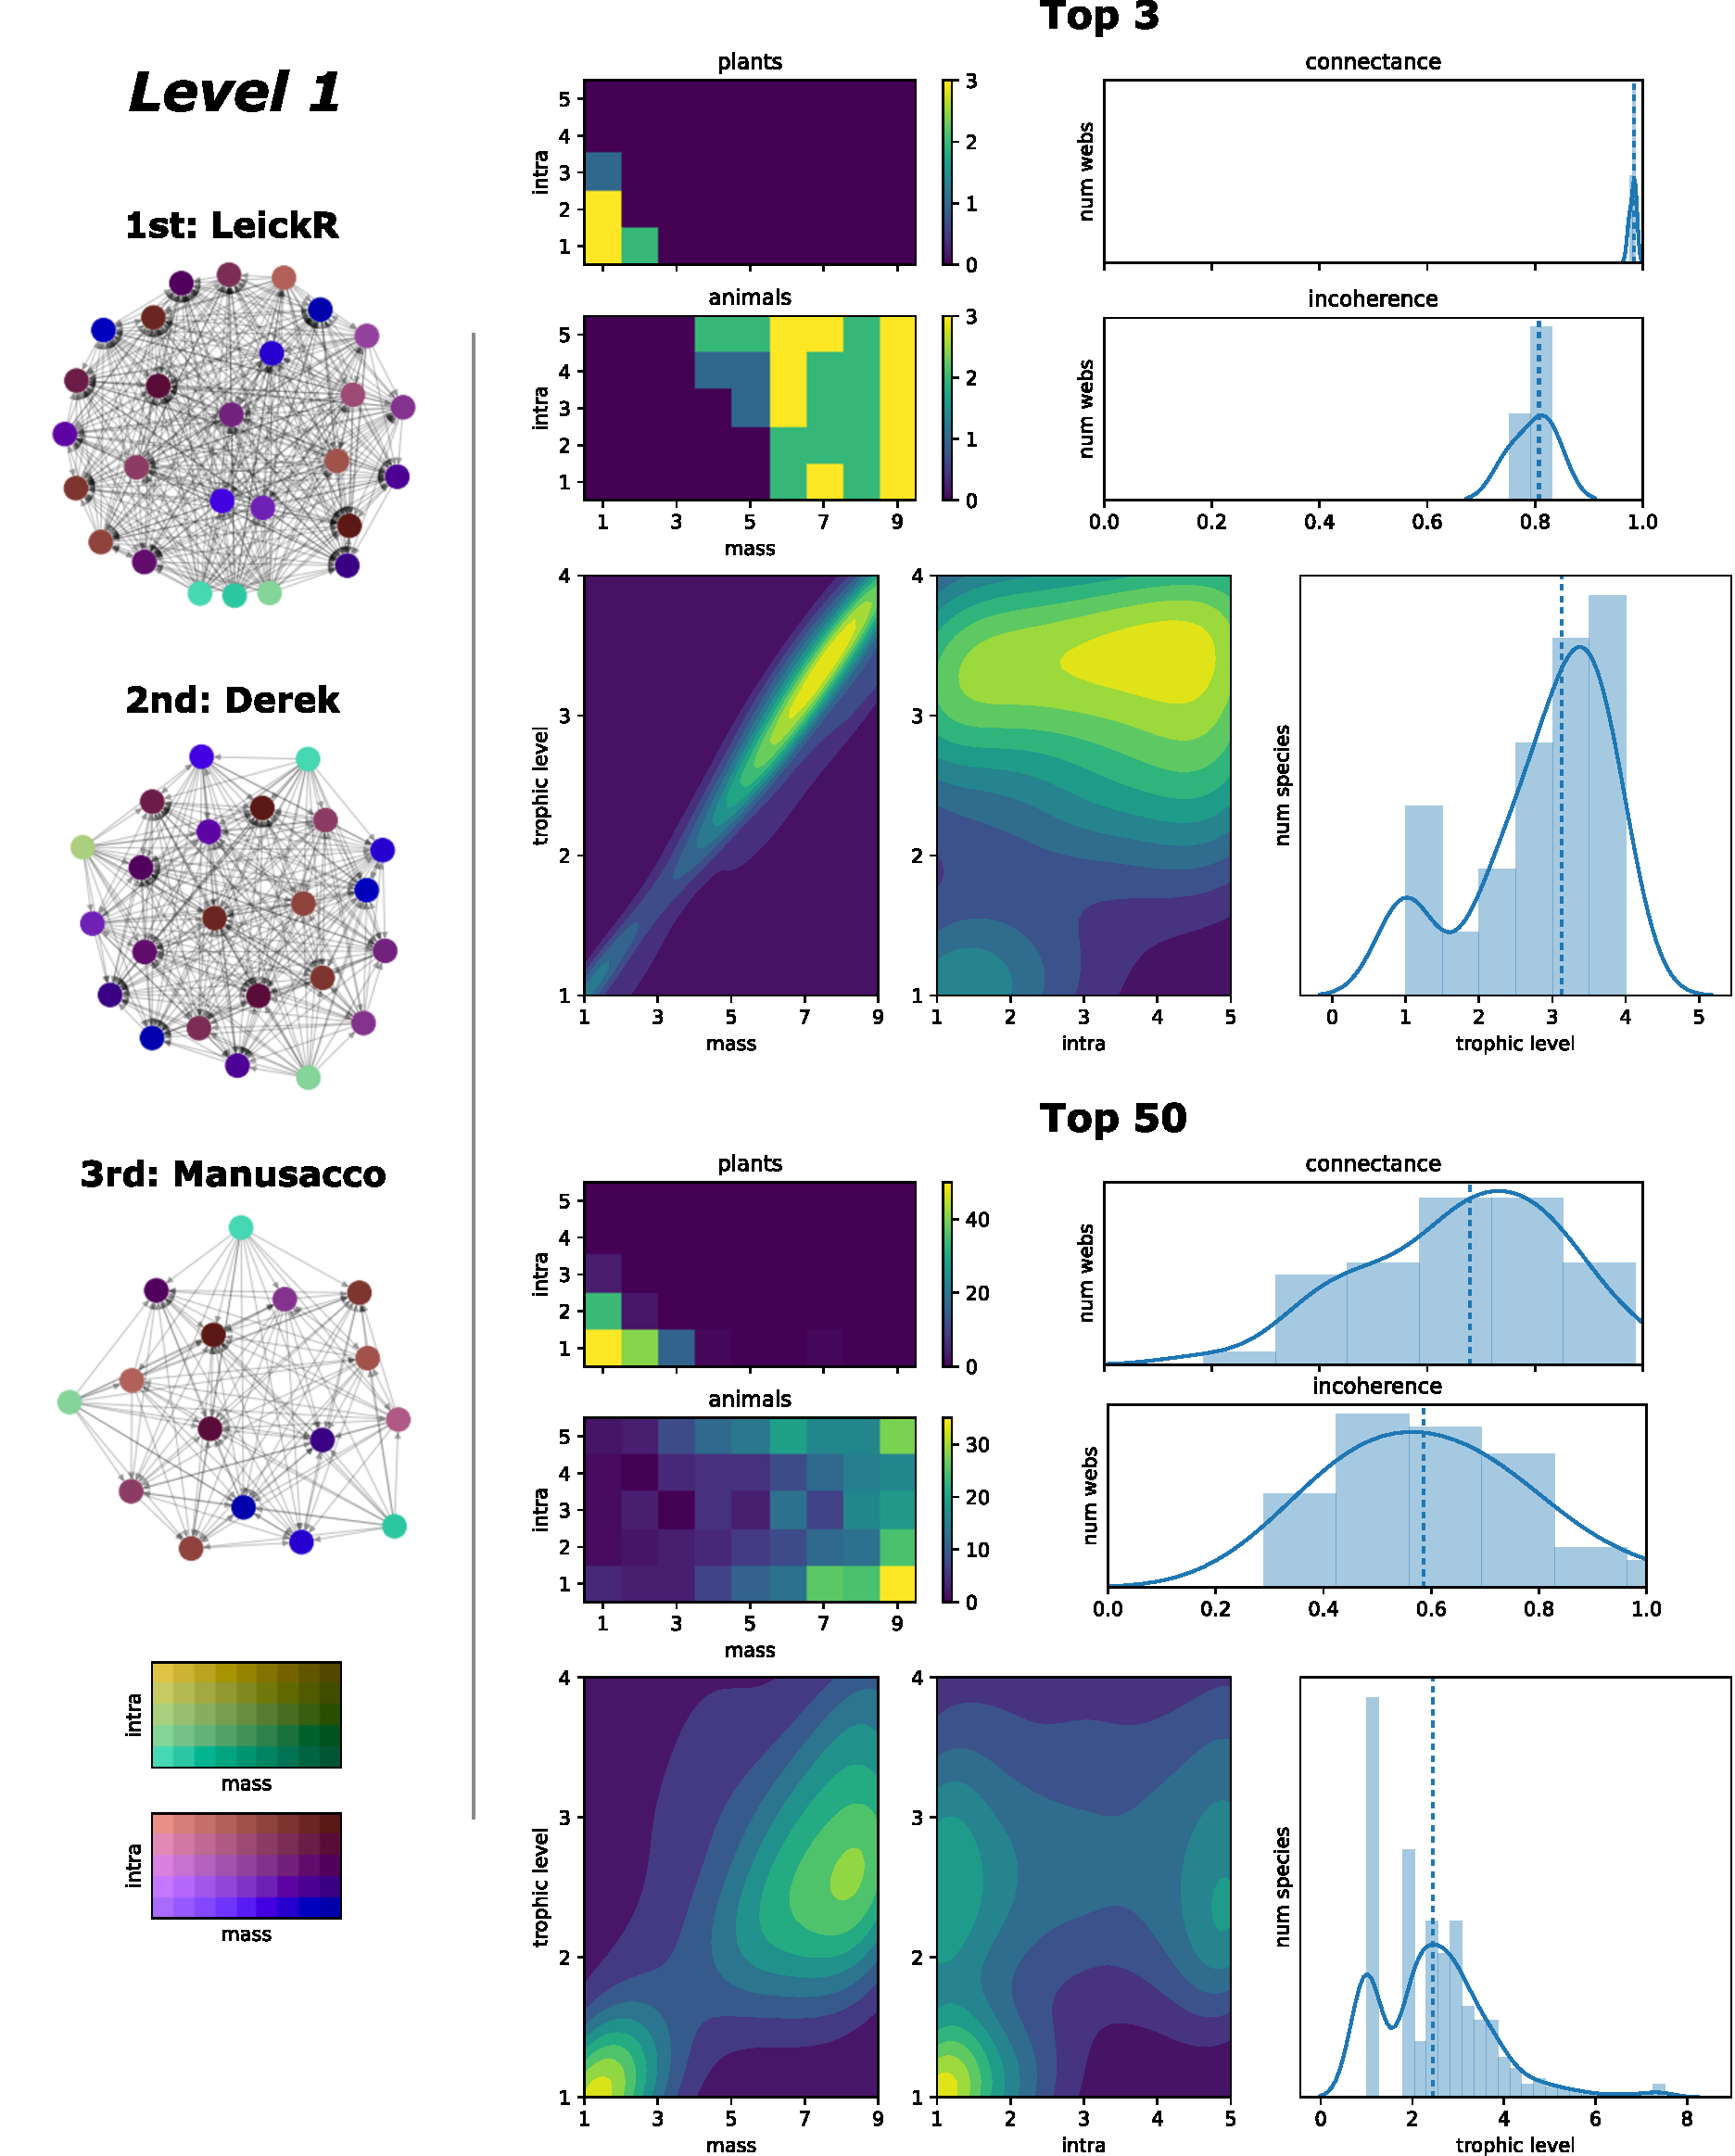
\includegraphics[height=.85\textheight, right]{joy/101.pdf}
  \caption[Results from Research World level 1]{An analysis of strategies used for level 1 of Research world. On the left are layouts of the top 3 leaderboard scores, with a colour map to show the colours of trait combinations for plants and animals.
  To the top-right is an analysis of these three scores with various histograms. Counter-clockwise from the top-left: the number of plants with each possible combination of traits, the same but for animals, the masses and trophic level of each species, the same for intraspecific interference, trophic levels of all species, incoherence (Equation~\eqref{eq:coherence}), and connectance. On the bottom-right are the same plots, but for the top 50 scores.}
  \label{fig:101}
\end{figure}
\begin{figure}
  \centering
  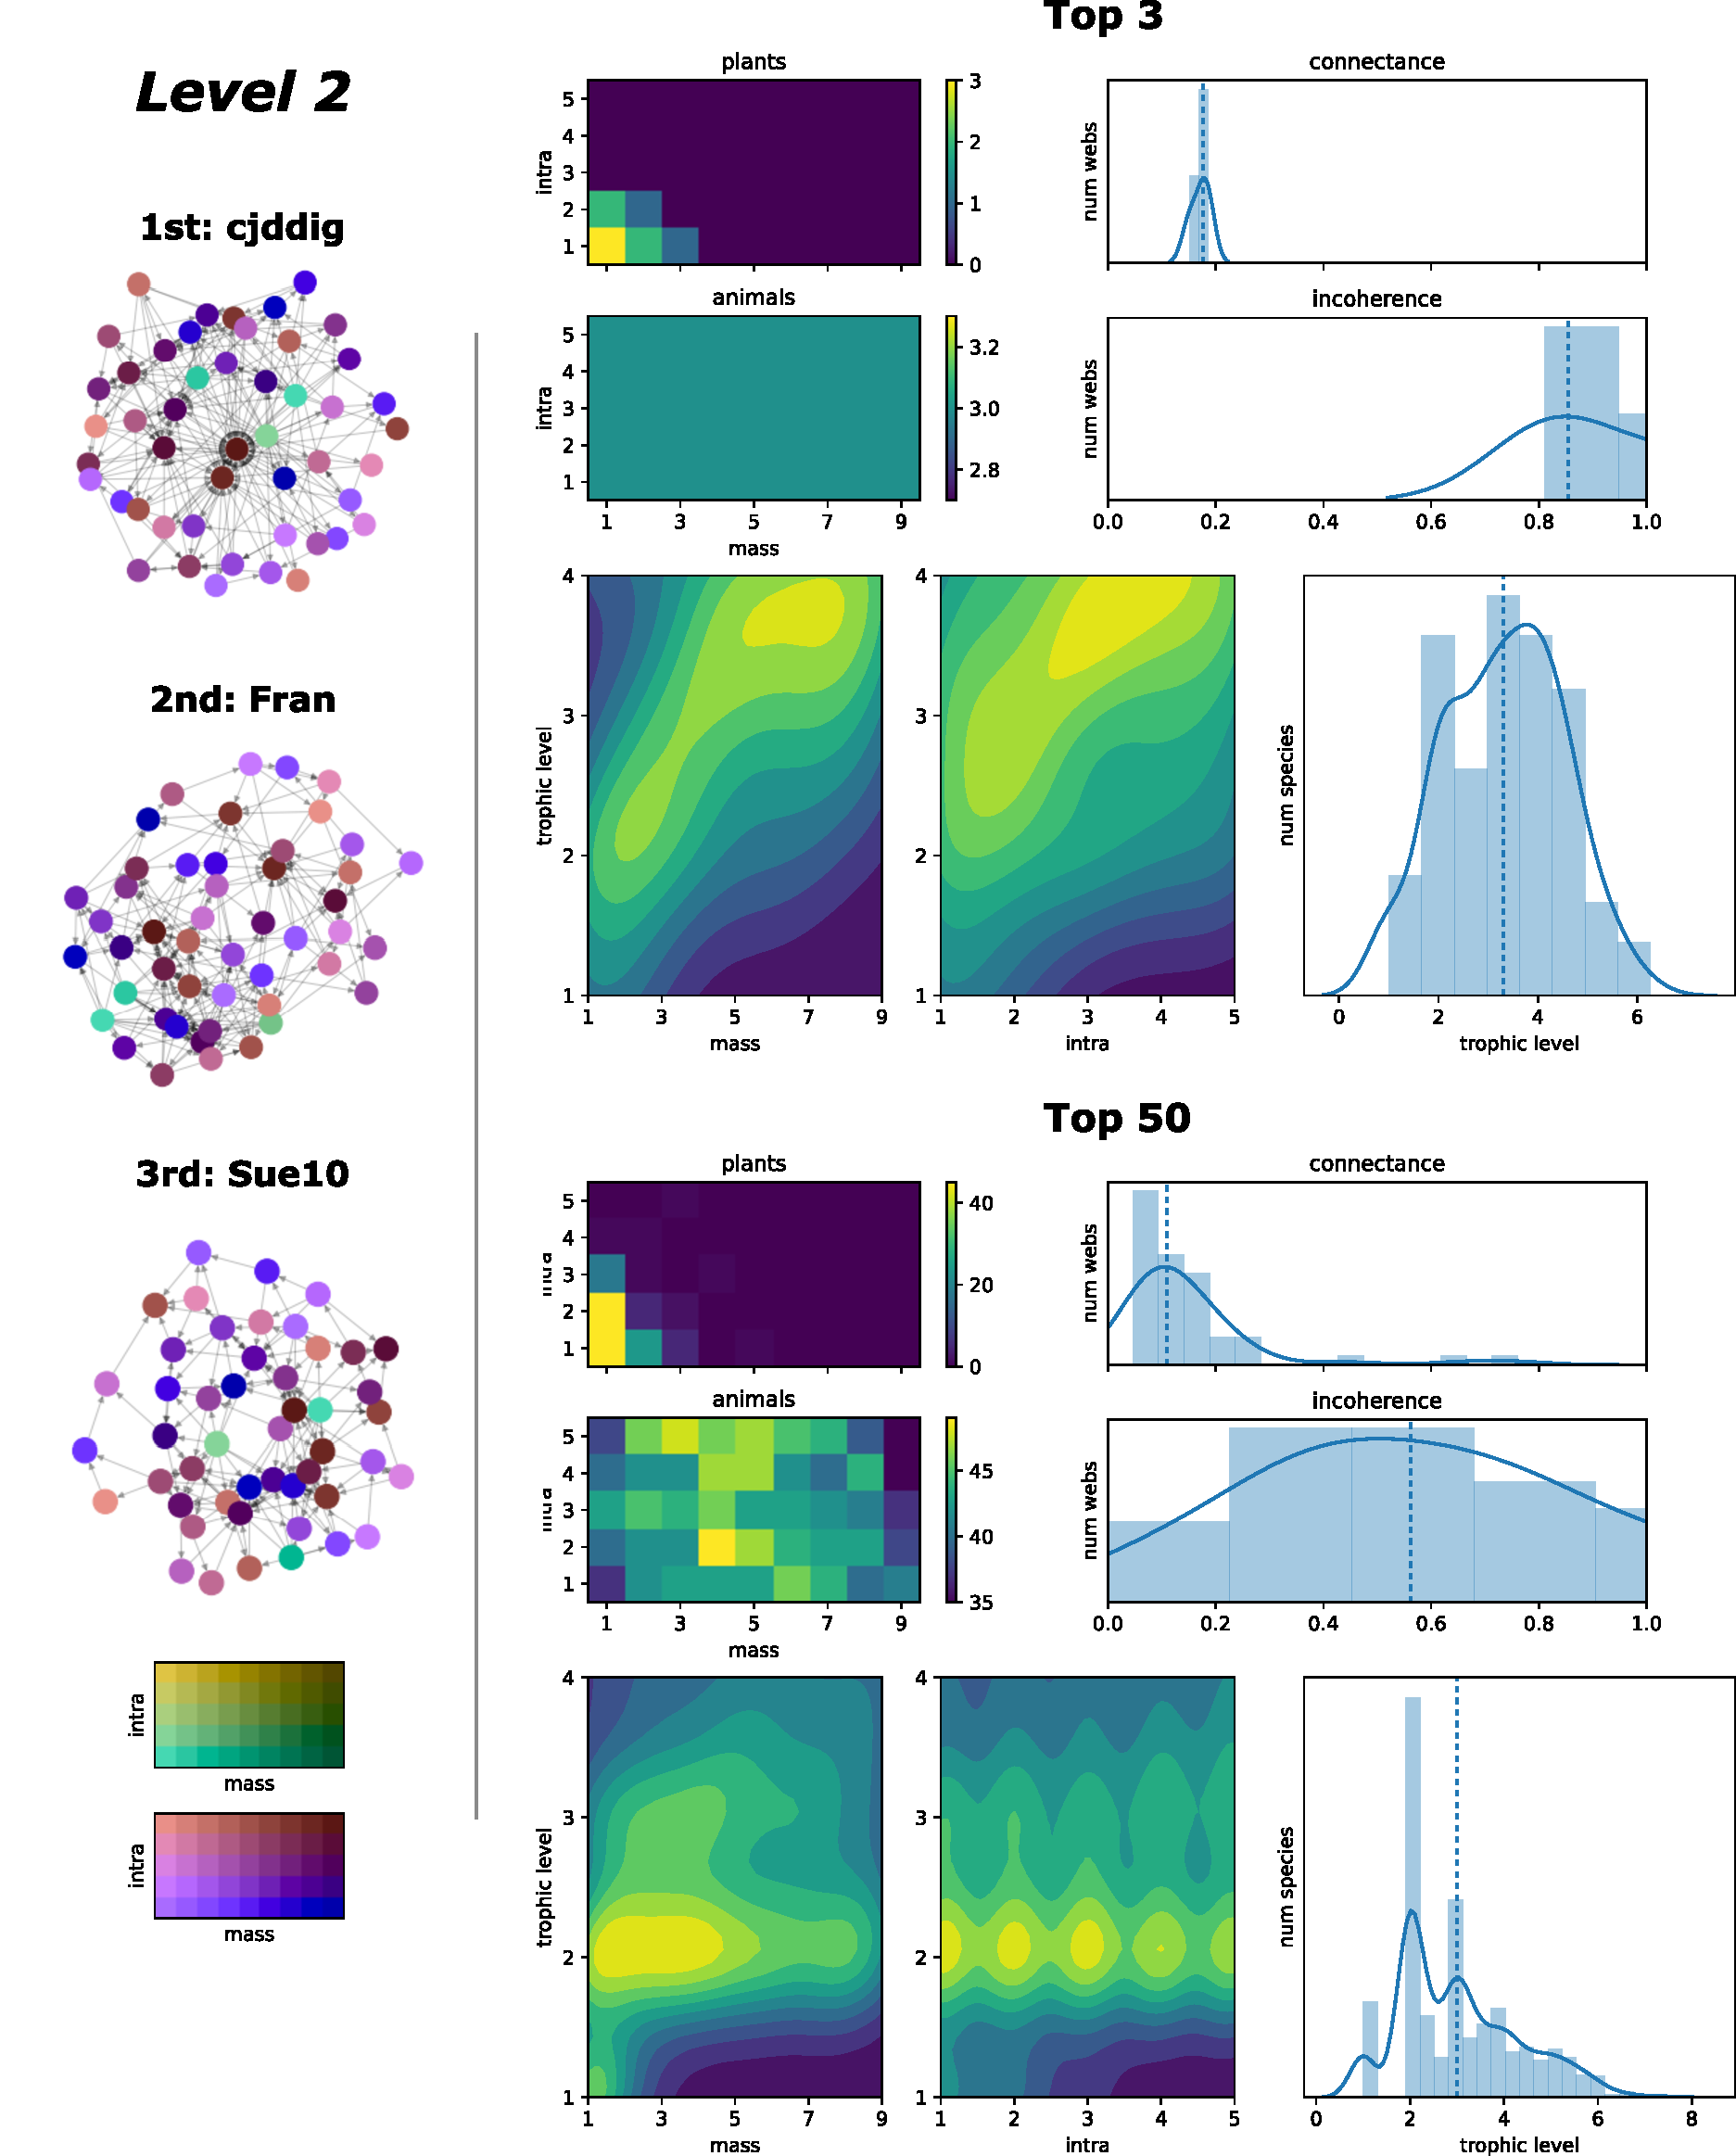
\includegraphics[height=.85\textheight, right]{joy/102.pdf}
  \caption[Results from Research World level 2]{An analysis of strategies used for level 2 of Research World, with the same conventions as Figure~\ref{fig:101}.}
  \label{fig:102}
\end{figure}
\begin{figure}
  \centering
  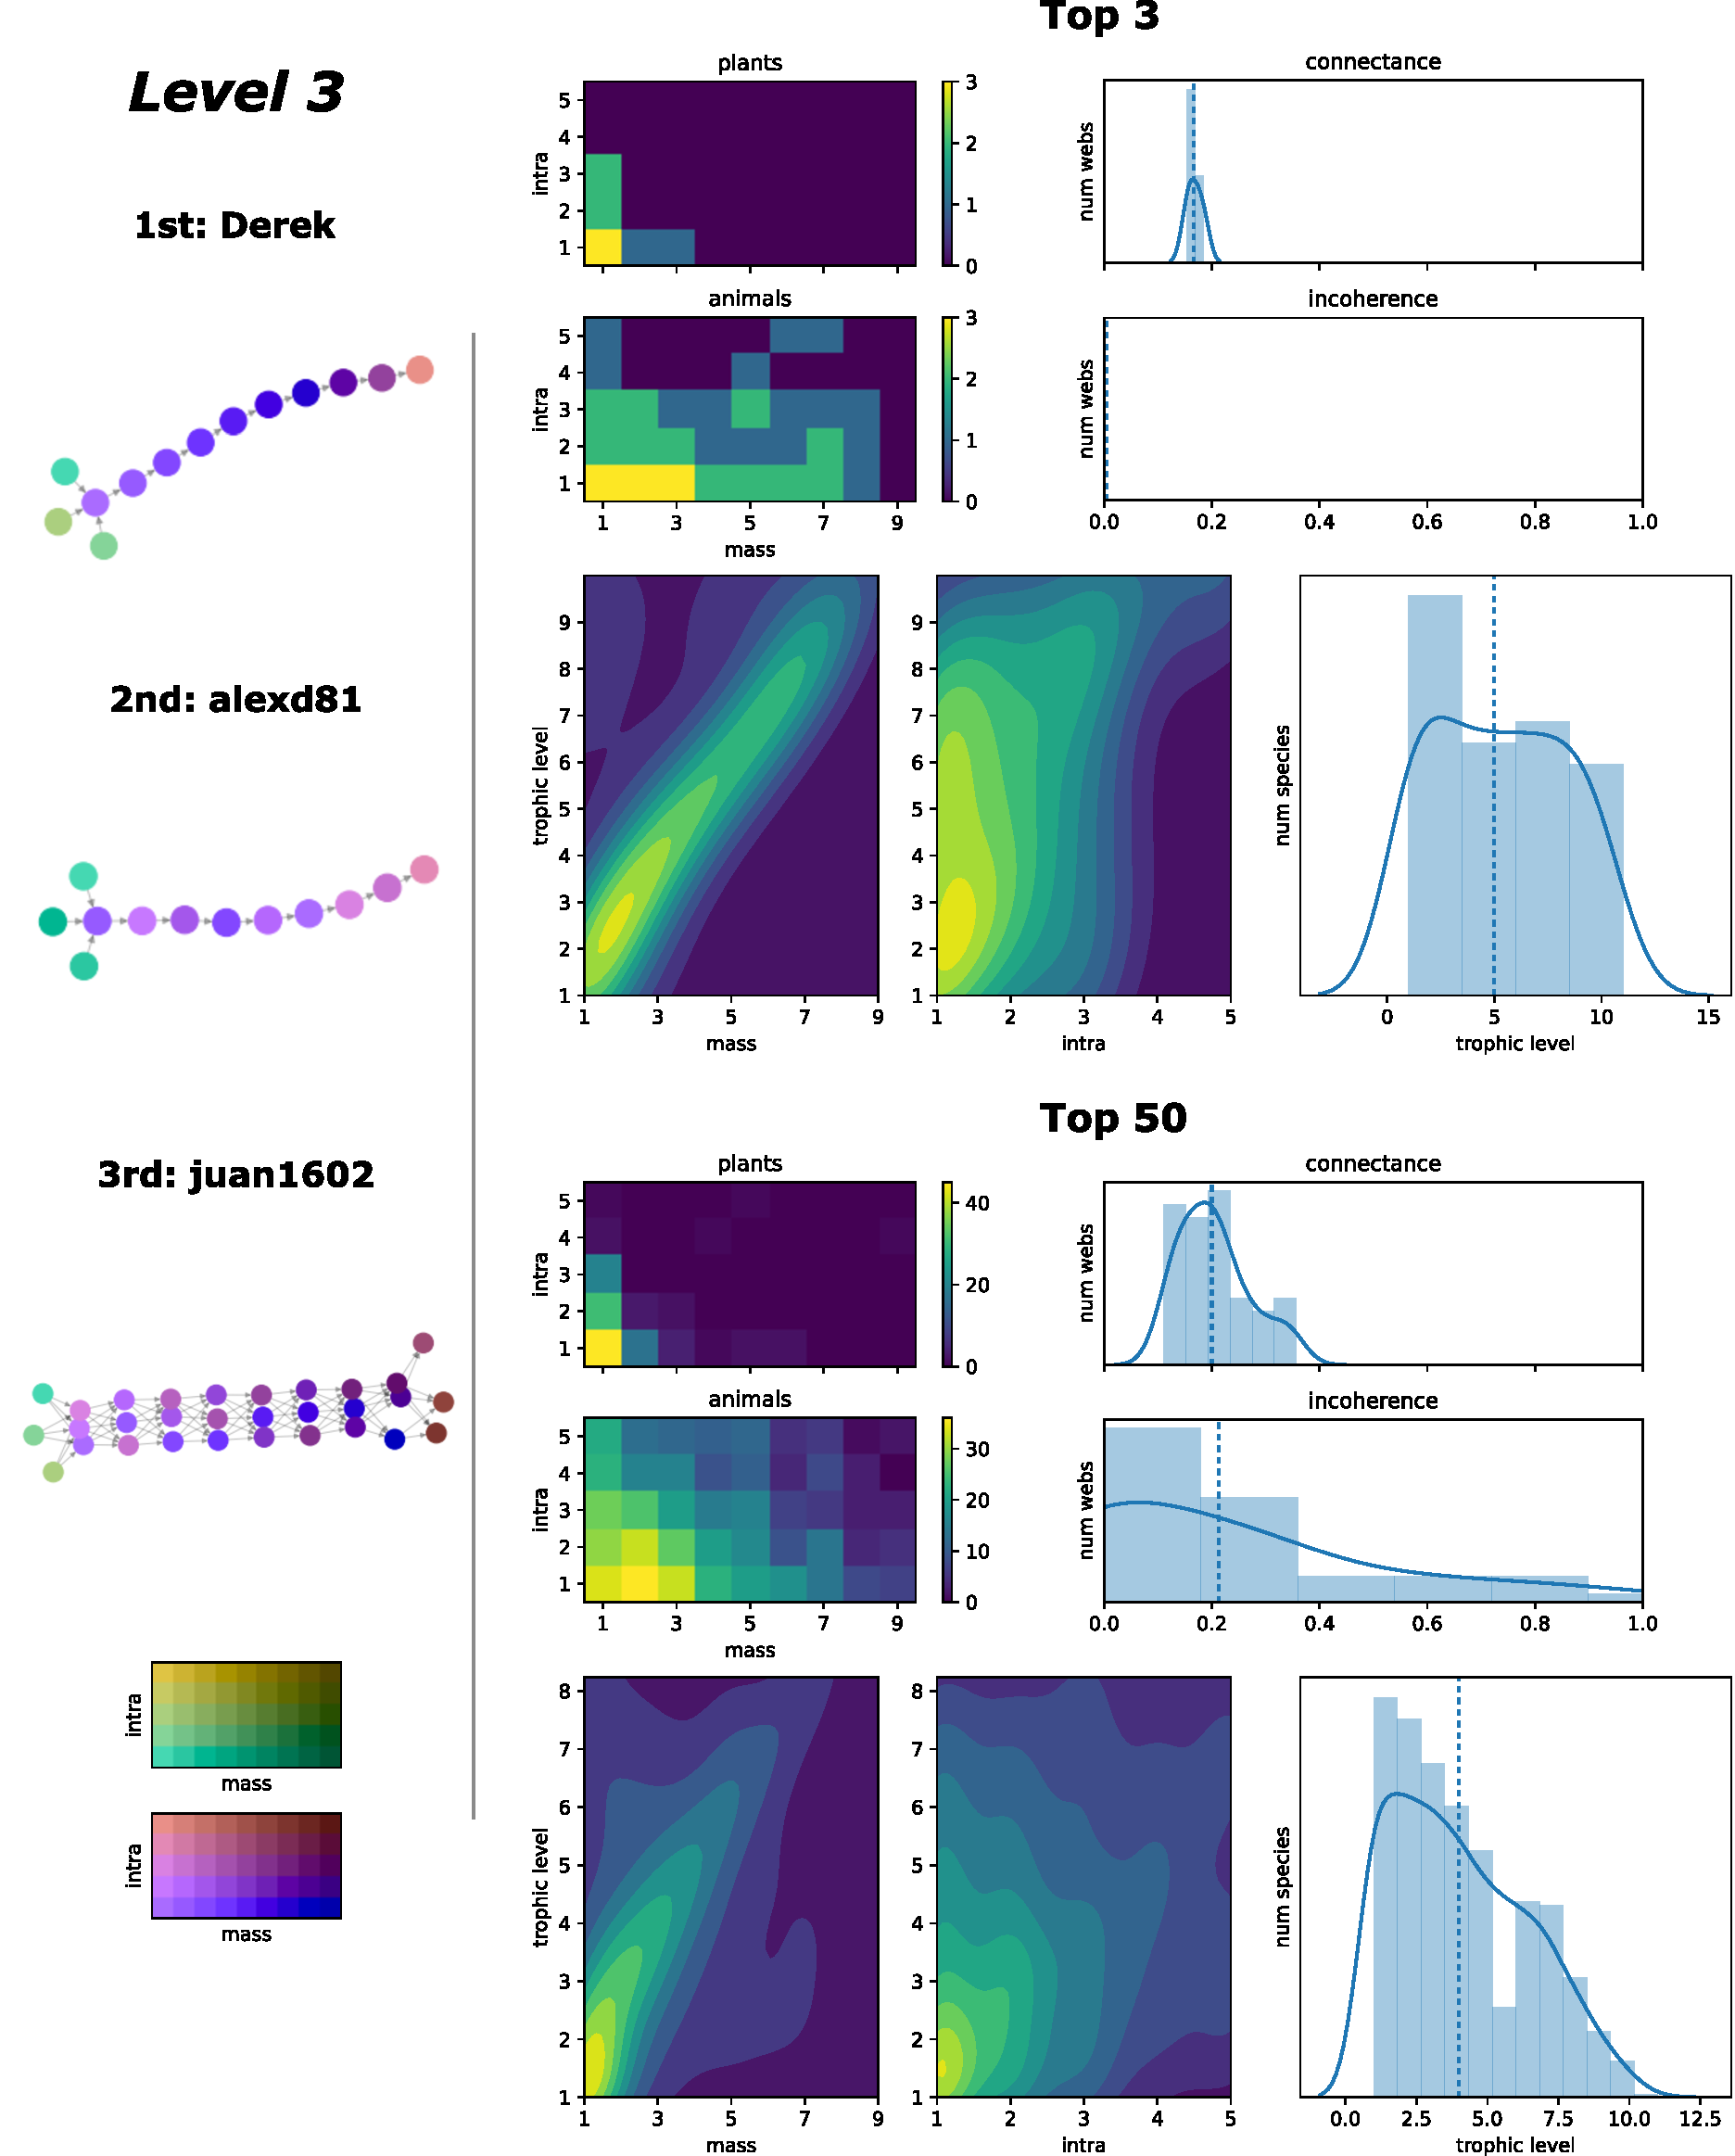
\includegraphics[height=.85\textheight, right]{joy/103.pdf}
  \caption[Results from Research World level 3]{An analysis of strategies used for level 3 of Research World, with the same conventions as Figure~\ref{fig:101}.}
  \label{fig:103}
\end{figure}
The food webs of the top three players are drawn on the left of each plots, along with their names. On the right of each plot are histograms plotting some features of these top three webs in the top half, and the same features on the top 50 scores on the bottom. The top half therefore shows the best of the best strategies, and the bottom shows the general patterns of all good strategies to place relatively highly on the leaderboards.

The three levels will be examined in succession, starting with level 1, where a very clear correlation of trophic to body mass is shown in the top 3 scores. This pattern is weaker but still present for the top 50 webs.
Connectance for level 1 is very high because the score metric (Equation~\eqref{eq:score}) demands it, and webs are in general incoherent. From this, it can be posited that a strong correlation between trophic level and body mass is necessary for webs with high connectance to be feasible.
% Another feature that is not immediate obvious is that the webs here must contain loops. This is because a high connectance implies that almost every species is eating every other species, and so the only way for trophic levels to get even close to three (and even four in some species here) is that loops are pushing up the trophic levels somewhere in the summation.
% Could possibly be a clue for omnivory.

Level 2 removes the need for high connectance, and it is clear that players took advantage of this, as the median connectance shot all the way down to below 0.2 for the best webs, and even lower over the top 50. This is strong evidence that high connectance webs are more difficult to build, which is in line with most predictions \cite{May1973,Allesina2012}.
In fact this is such a strong effect that, as shown by the completely flat histogram of animal traits, that the best players were able to make all 45 possible animals coexist. This is not only impressive, but also shows that building large and diverse ecosystems that are feasible is possible, given the right configurations.
As a caveat, the drop in connectance may also be a side-effect of high-connectance webs producing more cluttered visualisations, such that players may actively try to avoid them.
It is also of note that the the best webs in level 2 are very incoherent. This is a signal that there is a lot of omnivory in diverse ecosystems, which may suggest that omnivory plays a part in supporting large ecosystems.
% The same pattern of high trophic levels being correlated with high body masses exists here, as with level 1, although it is not as pronounced, which may mean that l.

Finally, the webs produced in level 3 are perhaps the least realistic, but are still insightful nonetheless. The best webs here show that for long chain lengths to exist, then coherence is likely to be necessary. The plot of mass and trophic levels shows the same pattern of heavier species at high trophic levels as before, but with more lighter species overall in the web than heavy. This is likely because lighter species are required to sustain high levels of biomass flow up to the next trophic level, and so more are needed to be a powerful `base' for the webs.
There is also a clear pattern in the trait combination plots, where most species, including animals, are concentrated around low mass and low interference. This is very different from the high connectance webs in level 1, where heavy species were preferred, and high interference is used as often as low. This is again likely because of the need for a large amount of biomass flowing up the lower levels.
% Therefore, another way of looking at level 3 is to see it as a level that forces maximal flux
% These results may also shed light upon the omnivory vs.\ coherence debate.

It is also clear from all levels that low mass and low interference is optimal for plants. This is relatively obvious, as it is the combination that results in the highest plant abundance. There is therefore no evidence that players ran into the `paradox of enrichment', that states that sometimes higher abundance of prey can destabilise webs \cite{Rosenzweig1971}.

The food webs built in Research World can also be used to examine the choice of range of interference strengths (diagonals in Equation~\eqref{eq:interaction_matrix}), which was 10$^{\text{--}4}$ to 10$^{\text{--}1}$. Looking at all off-diagonal values in all interaction matrices in the 3 Research levels shows that 95\% of the values lie in between the range 5$\times$10$^{\text{--}6}$ to 7$\times$10$^{\text{--}2}$. 
This range is in roughly line with the results of Ho \cite{Ho2020}, where it is shown that maximum feasibility in food webs occurs when the diagonals are around ten times larger than the off-diagonals.
% This is a chicken-and-egg problem, as it is not clear whether players subconsciously adapted to the range of interference strengths given to them, or if the choice was constrained into a good range in the first place.

\subsection{Discussion}
\label{sec:eco_discussion}

The work in this chapter has presented EcoBuilder: a video game for crowdsourcing mathematical ecology. It was publicly promoted from the 31st of July 2020, and the results here were taken from data collected up until the 16th of August, making up a span of one and a half months. Demographics for players of the game can be seen in Figure~\ref{fig:demo}.

\begin{figure}
  \centering
  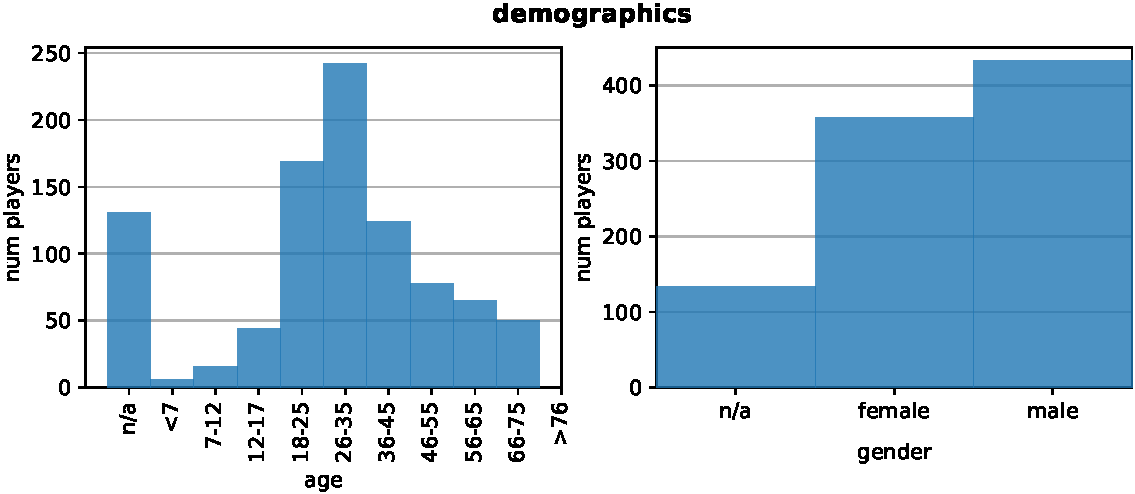
\includegraphics[width=\textwidth, right]{joy/demo.pdf}
  \caption[Player demographics]{Player demographics for EcoBuilder. Most players were ages in in the 20s to 30s, but with a good mix of other age groups too. Gender was also slightly more biased towards males, with no players picking a third `other' option.}
  \label{fig:demo}
\end{figure}

There were two research outcomes planed from the game. The first was a quantitative comparison of two different visualisations, where one is a standard layout and another has y-axis positions constrained.  The results of this are outlined in Section~\ref{sec:hypothesis1}, where it was shown that constraining the y-axis does make a small, but significant difference to many of the tasks performed in the game.
An older version of the game also planned to make use of the 3D capabilities of the Unity game engine, by placing species in three dimensions and having players rotate the resulting node-link diagram. However, early playtests revealed that players could not digest this interface easily, and so the game was converted back to 2D.

The second outcome was to have players tackle ecological puzzles where the solutions are far from clear, in an attempt to crowdsource the intelligence of humans for pattern recognition. It was hoped that a healthy dose of competition would motivate players to find structural patterns to build healthy ecosystems, and the results here show that this faith was well placed. Players exceeded expectations, especially on level two where many were able to make all possible species coexist.
The qualitative analysis presented in Section~\ref{sec:hypothesis2}, even as an exploratory and early stage study, revealed a number of patterns in player strategies, and a more precise dive into specific topologies of the top scores is sure to show even more.
It is clear that the general public are a powerful resource, and that they are more than happy to contribute when presented with a challenging but accessible opportunity to do so.
% With the growing democratisation of technology, it is an avenue that is more available than ever.

%   mention old idea for chess-board and why it didn't work
%      chess board not used anymore
%         We will use this result by restricting the player to an interface based on a two-dimensional niche space, presented as a board game not unlike chess, where pieces represent species and boxes will be drawn to decide what the species eats.

%         Why real food webs exhibit this low-dimensional structure is still up for debate, as it is unclear whether it is due to mechanistic environmental constraints (bottom-up control) or an emergent property of system stability (top-down control).
%         Either way for us it does not matter, because in the first case it means our restrictions are more realistic, and in the second case we are just helping the user towards stable configurations.
%         Our goal is to model the real world as close as possible, and that is what we are doing by restricting the structure; that it also keeps our interface for designing such structures scalable is a fortunate side-effect.

An important observation for future projects that involve interactive networks is that, on the small vertical screens of mobile devices, layouts can get very crowded with even a couple of dozen nodes.
Any sequel that would attempt to consider even larger ecosystems, i.e.\ in the order of hundreds of species, would be more suited to a desktop setting, and would likely require a more specialised visualisation than a standard force-directed layout.
Restricting the player to two-dimensional topologies, as defined in Section~\ref{sec:topology}, could offer a neat solution to the problem, as each species would only require a position, along with two coordinates to specify its feeding range, to fully describe its incoming links.
Edge bundling techniques like those studied in Chapter~\ref{chap:power} were also deemed as too complex for the context of a mobile game, but a desktop version could open that door as well.

All source code and assets used to produce the game are open source and publicly available at \url{www.github.com/jxz12/EcoBuilder}.